\chapter[ESPACIOS VECTORIALES]{ESPACIOS \\ VECTORIALES}\label{chap:ev}
%\startcontents
\printchaptertableofcontents

En las páginas que siguen, exploraremos un concepto central y poderoso: los espacios vectoriales. Estas estructuras matemáticas son la base de numerosos campos científicos y tecnológicos, permitiéndonos comprender y resolver una amplia gama de problemas. En esta obra, aprenderemos qué es un espacio vectorial real, sus propiedades fundamentales y cómo se aplican en situaciones prácticas.

\section{Definición y ejemplos}

\begin{definition}\label{definicion:espvec}
    Sea $V$ un conjunto no vacío y sea $K$ un campo que llamaremos escalares. Definimos la suma de elementos en $V$ y una multiplicación por un escalar respectivamente, como\infoBulle{En la definición \ref{definicion:espvec}, en lugar de $K$ se puede colocar un campo arbitrario, por ejemplo $\QQ$ o $\CC$. En este caso decimos que $V$ es un espacio vectorial sobre $K$.}
    \begin{alignat*}{2}
        + &: & \quad V \times V & \longrightarrow V \\
        & & (\mathbb{u}, \mathbb{v}) & \longmapsto \mathbb{u} + \mathbb{v} \\
        & \\
        \cdot &: & \quad K \times V & \longrightarrow V \\
        & & (\alpha, \mathbb{u}) & \longmapsto \alpha \cdot \mathbb{u}
    \end{alignat*}
    Decimos que $V$ es un espacio vectorial sobre $K$, si cumple con los siguientes axiomas: Para toda $\mathbb{x}$, $\mathbb{y}$, $\mathbb{z} \in V$ y $\alpha$, $\beta \in K$
    \begin{enumerate}[label=\roman*)]
        \item Cerradura: $\mathbb{x} + \mathbb{y} \in V$.
        \item Asociatividad: $\mathbb{x} + (\mathbb{y} + \mathbb {z}) = (\mathbb{x} + \mathbb{y}) + \mathbb{z}$.\newpage
        \item Conmutatividad: $\mathbb{x} + \mathbb{y} = \mathbb{y} + \mathbb{x}$.
        \item Neutro aditivo: Existe un elemento $\mathbb{0} \in V$ que llamaremos cero tal que $\mathbb{x} + \mathbb{0} = \mathbb{0} + \mathbb{x} = \mathbb{x}$.
        \item Inverso aditivo: Para cada $\mathbb{x} \in V$, existe un elemento $-\mathbb{x} \in V$ tal que $\mathbb{x} + (-\mathbb{x}) = \mathbb{0}$. A $-\mathbb{x}$ se le llama inverso de $\mathbb{x}$.
        \item Cerradura: $\alpha \cdot \mathbb{x} \in V$.
        \item Asociatividad: $\alpha \cdot (\beta \cdot \mathbb{x}) = (\alpha \cdot \beta) \cdot \mathbb{x}$.
        \item Distributividad (con un escalar): $\alpha \cdot (\mathbb{x} + \mathbb{y}) = \alpha \mathbb{x} + \alpha \mathbb{y}$.
        \item Distributividad (con dos escalares): $(\alpha + \beta) \cdot \mathbb{x} = \alpha \mathbb{x} + \beta \mathbb{x}$.
        \item Identidad multiplicativa: $1 \cdot \mathbb{x} = \mathbb{x}$.
    \end{enumerate}
\end{definition}

\begin{convention}
A menos que se indique específicamente otra cosa, por un espacio vectorial, entenderemos un espacio vectorial sobre $\RR$.
\end{convention}

\begin{definition}
    Sea $V$ un espacio vectorial sobre $K = \RR$, a sus elementos se les llama \textbf{vectores}.
\end{definition}

\begin{theorem}[Unicidad del inverso y el neutro aditivo]
    En un espacio  vectorial $V$ sobre $K$, el inverso y el neutro aditivo son únicos. \\
    \demostracion
    Veamos primero que el neutro aditivo es único. Del axioma iv), existe $\mathbb{0} \in V$ tal que para toda $\mathbb{x} \in V$
    \begin{equation}
        \mathbb{x} + \mathbb{0} = \mathbb{0} + \mathbb{x} = \mathbb{x} \label{ec1}
    \end{equation}
    Supongamos que existe $\tilde{\mathbb{0}} \in V$ tal que
    \begin{equation}
        \mathbb{x} + \tilde{\mathbb{0}} = \tilde{\mathbb{0}} + \mathbb{x} = \mathbb{x} \label{ec2}
    \end{equation}
    de \eqref{ec1}, como se cumple para toda $\mathbb{x} \in V$, en particular se cumple para $\mathbb{x} = \tilde{\mathbb{0}}$, es decir
    \begin{equation}
        \tilde{\mathbb{0}} + \mathbb{0} = \mathbb{0} + \tilde{\mathbb{0}} = \tilde{\mathbb{0}} \label{ec3}
    \end{equation}
    de igual forma, de la expresión \eqref{ec2} se cumple para toda $\mathbb{x} \in V$, en particular, para $\mathbb{x} = \mathbb{0}$. Así
    \begin{equation}
        \mathbb{0} + \tilde{\mathbb{0}} = \tilde{\mathbb{0}} + \mathbb{0} = \mathbb{0} \label{ec4}
    \end{equation}
    de \eqref{ec4} y \eqref{ec3}
    \begin{equation*}
        \tilde{\mathbb{0}} \stackrel{\eqref{ec3}}{=} \mathbb{0} + \tilde{\mathbb{0}} \stackrel{\eqref{ec4}}{=} \mathbb{0}
    \end{equation*}
    Por tanto, $\tilde{\mathbb{0}} = \mathbb{0}$.

    
    Ahora, demostremos que el inverso es único. Del axioma v), tenemos que para cada $\mathbb{x} \in V$ existe $-\mathbb{x}$ tal que
    \begin{equation}
        \mathbb{x} + (-\mathbb{x}) = \mathbb{0} \label{ec5}
    \end{equation}
    Supongamos que existe $\bbeta \in V$ tal que
    \begin{equation}
        \mathbb{x} + \bbeta = \mathbb{0} \label{ec6}
    \end{equation}
    Demostraremos que $\bbeta = -\mathbb{x}$
    \begin{align*}
        \bbeta & = \bbeta + \mathbb{0} && \text{por axioma iv)} \\
        & = \bbeta + \big( \mathbb{x} + (-\mathbb{x}) \big) && \text{por axioma v)} \\
        & = (\bbeta + \mathbb{x}) + (-\mathbb{x}) && \text{por axioma ii)} \\
        & = (\mathbb{x} + \bbeta) + (-\mathbb{x}) && \text{por axioma iii)} \\
        & = \mathbb{0} + (-\mathbb{x}) && \text{por la expresión \eqref{ec6}} \\
        & = -\mathbb{x} && \text{por axioma iv)}
    \end{align*}
    Por lo tanto, $\bbeta = -\mathbb{x}$.
\end{theorem}

\begin{theorem}
    Sea $V$ un espacio vectorial sobre $K$, entonces
    \begin{enumerate}[label=\roman*.]
        \item $\alpha \cdot \mathbb{0} = \mathbb{0}$, $\forall \alpha \in K$.
        \item $0 \cdot \mathbb{x} = \mathbb{0}$, $\forall \mathbb{x} \in V$.
        \item Si $\alpha \cdot \mathbb{x} = \mathbb{0}$, entonces $\alpha = 0$ o $\mathbb{x} = \mathbb{0}$.
        \item $(-1) \cdot \mathbb{x} = - \mathbb{x}$.
    \end{enumerate}
    \demostracion
    \begin{enumerate}[label=\roman*.]
        \item Sea $\alpha \in K$, tenemos que
        \begin{align}
            \mathbb{0} & = \mathbb{0} + \mathbb{0} && \text{por axioma iv)} \label{ec7} \\
            & = \alpha \cdot \mathbb{0} + (-\alpha \cdot \mathbb{0}) && \text{por axioma v)} \label{ec8}
        \end{align}
        de \eqref{ec7},
        \begin{align}
            \alpha \cdot \mathbb{0} & = \alpha \cdot (\mathbb{0} + \mathbb{0}) && \text{por def. de producto escalar} \label{ec9} \\
            & = \alpha \cdot \mathbb{0} + \alpha \cdot \mathbb{0} && \text{por axioma viii)} \label{ec10}
        \end{align}
        sustituyendo \eqref{ec10} en la ecuación \eqref{ec8}, obtenemos
        \begin{align*}
            \mathbb{0} & = (\alpha \cdot \mathbb{0} + \alpha \cdot \mathbb{0}) + (-\alpha \cdot \mathbb{0}) \\
            & = \alpha \cdot \mathbb{0} + \big( \alpha \cdot \mathbb{0} + (-\alpha \cdot \mathbb{0}) \big) && \text{por axioma ii)} \\
            & = \alpha \cdot \mathbb{0} + \mathbb{0} && \text{por axioma v)} \\
            & = \alpha \cdot \mathbb{0} && \text{por axioma iv)}
        \end{align*}
        Por tanto, $\alpha \cdot \mathbb{0} = \mathbb{0}$.
        \item Sea $\mathbb{x} \in V$. Sabemos que en $K = \RR$, se cumple que $0 + 0 = 0$, ahora
        \begin{align}
            0 \cdot \mathbb{x} & = (0 + 0) \cdot \mathbb{x} && \text{por def. de producto escalar} \label{ec11} \\
            & = 0 \cdot \mathbb{x} + 0 \cdot \mathbb{x} && \text{por ix)} \label{ec12}
        \end{align}
        Por otra parte,
        \begin{align}
            \mathbb{0} & = 0 \cdot \mathbb{x} + (-0 \cdot \mathbb{x}) && \text{por axioma v)} \label{ec13}
        \end{align}
        Sustituyendo \eqref{ec12} en \eqref{ec13},
        \begin{align*}
            \mathbb{0} & = (0 \cdot \mathbb{0} + 0 \cdot \mathbb{0}) + (-0 \cdot \mathbb{x}) \\
            & = 0 \cdot 0 + \big( 0 \cdot \mathbb{x} + (-0 \cdot \mathbb{x}) \big) && \text{por axioma ii)} \\
            & = 0 \cdot \mathbb{x} + 0 && \text{por axioma v)} \\
            & = 0 \cdot \mathbb{x} && \text{por axioma iv)}
        \end{align*}
        Por tanto, $0 \cdot \mathbb{x} = \mathbb{0}$.
        \item Supongamos que $\alpha \neq 0$, entonces hay que demostrar que $\mathbb{x} = \mathbb{0}$. Como $\alpha \in K$ y $\alpha \neq 0$, entonces existe $\alpha^{-1} \in K$ tal que
        \begin{equation}
            \alpha^{-1} \cdot \alpha = 1 \label{ec14}
        \end{equation}
        De la hipótesis,
        \begin{align*}
            \mathbb{0} & = \alpha^{-1} \cdot \mathbb{0} && \text{por (i) de este teorema} \\
            & = \alpha^{-1} \cdot (\alpha \cdot \mathbb{x}) && \text{por hipótesis} \\
            & = (\alpha^{-1} \cdot \alpha) \cdot \mathbb{x} && \text{por axioma vii)} \\
            & = 1 \cdot \mathbb{x} && \text{por ecuación \eqref{ec14}} \\
            & = \mathbb{x} && \text{por axioma x)}
        \end{align*}
        Por tanto, $\mathbb{x} = \mathbb{0}$.
        
        Ahora, supongamos que $\mathbb{x} = \mathbb{0}$. Procedamos por reducción al absurdo, supongamos que $\alpha \neq 0$, entonces existe $\alpha^{-1} \in K$ tal que \begin{equation}
            \alpha^{-1} \cdot \alpha = 1 \label{ec15}
        \end{equation}
        Entonces
        \begin{align*}
            \mathbb{x} & = 1 \cdot \mathbb{x} && \text{por axioma x)} \\
            & = (\alpha^{-1} \cdot \alpha) \cdot \mathbb{x} && \text{por la ecuación \eqref{ec15}} \\
            & = \alpha^{-1} \cdot (\alpha \cdot \mathbb{x}) && \text{por axioma vii)} \\
            & = \alpha^{-1} \cdot \mathbb{0} && \text{por hipótesis} \\
            & = \mathbb{0}
        \end{align*}
        Por lo tanto, $\mathbb{x} = \mathbb{0}$, que es lo que se quería demostrar. Ahora, si $\alpha = 0$ y $\mathbb{x} = \mathbb{0}$ la propiedad (iii) queda demostrada por los incisos (i) y (ii) de este teorema.
        \item Como
        \begin{equation}
            0 = 1 + (-1) \in K \label{ec16}
        \end{equation}
        por (i) de este teorema,
        \begin{align*}
            \mathbb{0} & = 0 \cdot \mathbb{x} \\
            & = \big( 1 + (-1) \big) \cdot \mathbb{x} && \text{por la expresión \eqref{ec16}} \\
            & = 1 \cdot x +  (-1) \cdot \mathbb{x} && \text{por axioma ix)}
        \end{align*}
        esto es
        \begin{equation}
            \mathbb{0} = 1 \cdot \mathbb{x} + (-1) \cdot \mathbb{x} \label{ec17}
        \end{equation}
        Ahora,
        \begin{align*}
            -\mathbb{x} & = - \mathbb{x} + \mathbb{0} \\
            & = -\mathbb{x} + \big( 1 \cdot \mathbb{x} + (-1) \cdot \mathbb{x} \big) && \text{por la expresión \eqref{ec17}} \\
            & = (-\mathbb{x} + 1 \cdot \mathbb{x}) + (-1) \cdot \mathbb{x} && \text{por axioma ii)} \\
            & = (-\mathbb{x} + \mathbb{x}) + (-1) \cdot \mathbb{x} && \text{por axioma x)} \\
            & = \mathbb{0} + (-1) \cdot \mathbb{x} && \text{por axioma v)} \\
            & = (-1) \cdot \mathbb{x} && \text{por axioma iv)}
        \end{align*}
        Por tanto, $-\mathbb{x} = (-1) \cdot \mathbb{x}$.
    \end{enumerate}
\end{theorem}

\begin{example}
    Recordemos por el curso de Geometría Analítica que
    $$\RR[2] = \left\{ \binom{x}{y} \mid x \in \RR, y \in \RR \right\}$$
    en el cual se definen dos operaciones dados $\mathbb{x}$, $\mathbb{y} \in \RR[2]$ con $\displaystyle \mathbb{x} = \binom{a}{b}$ e $\displaystyle \mathbb{y} = \binom{c}{d}$
    \begin{alignat*}{2}
        + &: & \quad \RR[2] \times \RR[2] & \longrightarrow \RR[2] \\
        & & ( \mathbb{x}, \mathbb{y} ) & \longmapsto \binom{a+c}{b+d} \\
        & \\
        \cdot &: & \quad \RR \times \RR[2] & \longrightarrow \RR[2] \\
        & & ( \alpha, \mathbb{x}) & \longmapsto \binom{\alpha a}{\alpha b}
    \end{alignat*}
    Notemos que las operaciones antes mencionadas admiten una interpretación geométrica. Vea la figura \ref{JAJAJJAJS} y \ref{UAIIOPOUSJSJ}.\sideFigure[\label{JAJAJJAJS}Representación geométrica de la operación $+$]{
    \begin{center}
        \begin{tikzpicture}[scale=0.83]
            \draw[thick,-Stealth] (-1,0) -- (5,0);
            \draw[thick,-Stealth] (0,-1) -- (0,5);
            \draw[dash pattern=on 3pt off 3pt] (1,3) -- (4,4) -- (3,1);
            \draw[dash pattern=on 3pt off 3pt] (0,4) -- (4,4) -- (4,0);
            \draw[dash pattern=on 3pt off 3pt] (0,3) -- (1,3) -- (1,0);
            \draw[dash pattern=on 3pt off 3pt] (0,1) -- (3,1) -- (3,0);
            \draw[-latex] (0,0) -- (3,1);
            \draw[-latex] (0,0) -- (1,3);
            \draw[-latex] (0,0) -- (4,4);
            \node at (0,4) [left] {$b+d$};
            \node at (0,3) [left] {$d$};
            \node at (0,1) [left] {$b$};
            \node at (1,0) [below] {$c$};
            \node at (3,0) [below] {$a$};
            \node at (4,0) [below] {$a+c$};
            \node at (4,4) [right] {$\displaystyle \begin{pmatrix} a + c \\ b + d \end{pmatrix}$};
        \end{tikzpicture}
    \end{center}
    }
    \sideFigure[\label{UAIIOPOUSJSJ}Representación geométrica de la operación $\cdot$]{
    \begin{center}
        \begin{tikzpicture}[scale=0.83]
            \draw[thick,-Stealth] (-1,0) -- (5,0);
            \draw[thick,-Stealth] (0,-1) -- (0,5);
            \draw[dash pattern=on 3pt off 3pt] (0,2) -- (2,2) -- (2,0);
            \draw[dash pattern=on 3pt off 3pt] (0,4) -- (4,4) -- (4,0);
            \draw[thick,-latex] (0,0) -- (4,4);
            \draw[thick,-latex] (0,0) -- (2,2);
            \node at (4,4) [right] {$\displaystyle \begin{pmatrix} \alpha a \\ \alpha b \end{pmatrix}$};
            \node at (2,1.8) [right] {$\displaystyle \begin{pmatrix} a \\ b \end{pmatrix}$};
            \node at (0,4) [left] {$\alpha b$};
            \node at (0,2) [left] {$b$};
            \node at (2,0) [below] {$a$};
            \node at (4,0) [below] {$\alpha a$};
        \end{tikzpicture}
    \end{center}
    }
    \newpage
    El conjunto $\RR[2]$ representa el conjunto de todos los pares ordenados de números reales. $\RR[2]$ es bidimensional, lo que significa que tiene dos dimensiones: la dimensión horizontal (eje $x$ por convención) y la dimensión vertical (eje $y$ por convención). En geometría analítica, se utiliza para representar figuras geométricas, ecuaciones de rectas, círculos y cualquier otra forma bidimensional.
    
    Probemos que $V = \RR[2]$, con las operaciones $+$ y $\cdot$ definidas previamente es un espacio vectorial sobre $\RR$. Verifiquemos los 10 axiomas de un espacio vectorial (definición \ref{definicion:espvec}) como sigue:
    \begin{enumerate}[label=\roman*)]
        \item Sea $\mathbb{x}$, $\mathbb{y} \in \RR[2]$ con $\displaystyle \mathbb{x} = \binom{a}{b}$, $\displaystyle \mathbb{y} = \binom{c}{d}$, entonces
        \begin{align*}
            \mathbb{x} + \mathbb{y} & = \binom{a}{b} + \binom{c}{d} \\
            & = \binom{a+c}{b+d} && \text{por def. de suma} \\
            & = \binom{a+c}{b+d} \in \RR[2]
        \end{align*}
        Ya que $a$, $b$, $c$, $d \in \RR$, entonces $a+c$, $b+d \in \RR$. Por tanto, se cumple la propiedad de cerradura.
        \item Sea $\mathbb{x}$, $\mathbb{y}$, $\mathbb{z} \in \RR[2]$ con $\displaystyle \mathbb{x} = \binom{a}{b}$, $\displaystyle \mathbb{y} = \binom{c}{d}$, $\displaystyle \mathbb{z} = \binom{m}{l}$, entonces
        \begin{align*}
            \mathbb{x} + (\mathbb{y} + \mathbb{z}) & = \binom{a}{b} + \left[ \binom{c}{d} + \binom{m}{l} \right] \\
            & = \binom{a}{b} + \binom{c+m}{d+l} && \text{por def. de suma} \\
            & = \binom{a+(c+m)}{b+(d+l)} && \text{por def. de suma} \\
            & = \binom{(a+c)+m}{(b+d)+l} && \text{por asociatividad en $\RR$} \\
            & = \binom{a+c}{b+d} + \binom{m}{l} && \text{por def. de suma} \\
            & = \left[ \binom{a}{b} + \binom{c}{d} \right] + \binom{m}{l} && \text{por def. de suma} \\
            & = (\mathbb{x} + \mathbb{y}) + \mathbb{z}
        \end{align*}
        Por tanto, se cumple la asociatividad.
        \item Sea $\mathbb{x}$, $\mathbb{y} \in \RR[2]$ con $\displaystyle \mathbb{x} = \binom{a}{b}$, $\displaystyle \mathbb{y} = \binom{c}{d}$, entonces
        \begin{align*}
            \mathbb{x} + \mathbb{y} & = \binom{a}{b} + \binom{c}{d} \\
            & = \binom{a+c}{b+d} && \text{por def. de suma} \\
            & = \binom{c+a}{d+b} && \text{por conmutatividad en $\RR$} \\
            & = \binom{c}{d} + \binom{a}{b} && \text{por def. de suma} \\
            & = \mathbb{y} + \mathbb{x}
        \end{align*}
        Por tanto, se cumple la conmutatividad.
        \item Sea $\mathbb{0} \in \RR[2]$ con $\displaystyle \mathbb{0} = \binom{0}{0}$, entonces
        \begin{align*}
            \mathbb{0} + \mathbb{x} & = \binom{0}{0} + \binom{a}{b} \\
            & = \binom{0+a}{0+b} && \text{por def. de suma} \\
            & = \binom{a}{b} && \text{por neutro aditivo en $\RR$} \\
            & = \mathbb{x}
        \end{align*}
        Por tanto, se cumple la propiedad del neutro aditivo.
        \item Dado $\displaystyle \mathbb{x} = \binom{a}{b}$, existe $\displaystyle -\mathbb{x} = \binom{-a}{-b} \in \RR[2]$ tal que
        \begin{align*}
            \mathbb{x} + (-\mathbb{x}) & = \binom{a}{b} + \binom{-a}{-b} \\
            & = \binom{a+(-a)}{b+(-b)} && \text{por def. de suma} \\
            & = \binom{a-a}{b-b} && \text{por definición en $\RR$} \\
            & = \binom{0}{0} && \text{por inv. aditivo en $\RR$} \\
            & = \mathbb{0}
        \end{align*}
        Por tanto, se cumple la propiedad del inverso aditivo.
        \item Sea $\alpha \in \RR$ y sea $\mathbb{x} \in \RR[2]$ con $\displaystyle \mathbb{x} = \binom{a}{b}$, entonces
        \begin{align*}
            \alpha \cdot \mathbb{x} & = \alpha \cdot \binom{a}{b} \\
            & = \binom{\alpha a}{\alpha b} \in \RR[2] && \text{por def. de producto}
        \end{align*}
        Ya que $\alpha a$, $\alpha b \in \RR$, se cumple la propiedad de cerradura.
        \item Sea $\alpha$, $\beta \in \RR$ y sea $\mathbb{x} \in \RR[2]$ con $\displaystyle \mathbb{x} = \binom{a}{b}$, entonces
        \begin{align*}
            \alpha \cdot (\beta \cdot \mathbb{x}) & = \alpha \cdot \left[ \beta \cdot \binom{a}{b} \right] \\
            & = \alpha \cdot \left[ \binom{\beta a}{\beta b} \right] && \text{por def. de producto} \\
            & = \binom{\alpha (\beta a)}{\alpha (\beta b)} && \text{por def. de producto} \\
            & = \binom{(\alpha\beta)a}{(\alpha\beta)b} && \text{por asociatividad en $\RR$} \\
            & = (\alpha\beta) \cdot \binom{a}{b} && \text{por def. de producto} \\
            & = (\alpha\beta) \cdot \mathbb{x}
        \end{align*}
        Por tanto, se cumple la asociatividad.
        \item Sea $\alpha \in \RR$ y sean $\mathbb{x}$, $\mathbb{y} \in \RR[2]$ con $\displaystyle \mathbb{x} = \binom{a}{b}$ e $\displaystyle \mathbb{y} = \binom{c}{d}$, entonces
        \begin{align*}
            \alpha \cdot (\mathbb{x} + \mathbb{y}) & = \alpha \cdot \left[ \binom{a}{b} + \binom{c}{d} \right] \\
            & = \alpha \cdot \binom{a+c}{b+d} && \text{por def. de suma} \\
            & = \binom{\alpha (a+c)}{\alpha (b+d)} && \text{por def. de producto} \\
            & = \binom{\alpha a + \alpha c}{\alpha b + \alpha d} && \text{por distributividad en $\RR$} \\
            & = \binom{\alpha a}{\alpha c} + \binom{\alpha b}{\alpha d} && \text{por def. de suma} \\
            & = \alpha \cdot \binom{a}{b} + \alpha \cdot \binom{c}{d} && \text{por def. de producto} \\
            & = \alpha \cdot \mathbb{x} + \alpha \cdot \mathbb{y}
        \end{align*}
        Por tanto, se cumple la distributividad con dos vectores y un escalar.
        \item Sean $\alpha$, $\beta \in \RR$ y sea $\mathbb{x} \in \RR[2]$ con $\displaystyle \mathbb{x} = \binom{a}{b}$, entonces
        \begin{align*}
            (\alpha + \beta) \cdot \mathbb{x} & = (\alpha + \beta) \cdot \binom{a}{b} \\
            & = \binom{(\alpha+\beta)a}{(\alpha+\beta)b} && \text{por def. de producto} \\
            & = \binom{\alpha a+\beta a}{\alpha b+\beta b} && \text{por distributividad en $\RR$} \\
            & = \binom{\alpha a}{\alpha b} + \binom{\beta a}{\beta b} && \text{por def. de suma} \\
            & = \alpha \cdot \binom{a}{b} + \beta \cdot \binom{a}{b} && \text{por def. de producto} \\
            & = \alpha \cdot \mathbb{x} + \beta \cdot \mathbb{x}
        \end{align*}
        Por tanto, se cumple la distributividad con dos escalares y un vector.
        \item Sea $\mathbb{x} \in \RR[2]$ con $\displaystyle \mathbb{x} = \binom{a}{b}$, entonces
        \begin{align*}
            1 \cdot \mathbb{x} & = 1 \cdot \binom{a}{b} \\
            & = \binom{1 \cdot a}{1 \cdot b} && \text{por def. de producto} \\
            & = \binom{a}{b} && \text{por identidad multiplicactiva en $\RR$} \\
            & = \mathbb{x}
        \end{align*}
        Por tanto, se cumple la propiedad de identidad multiplicativa.
    \end{enumerate}
    Por lo tanto, $\RR[2]$ es un espacio vectorial sobre $\RR$.
\end{example}

$\RR[n]$ es un concepto matemático fundamental que representa un espacio vectorial de dimensión $n$ sobre los números reales $\RR$. En términos más simples, $\RR[n]$ es el conjunto de todos los vectores con $n$ componentes reales. Cada componente de un vector en $\RR[n]$ corresponde a una coordenada a lo largo de un eje específico en un espacio $n$-dimensional. En lugar de definir en este punto a $\RR[n]$, veamos algunos ejemplos para derivar la idea a partir de ellos. Por ejemplo, un número real $x$ puede ser representado por un punto sobre una línea.
\begin{figure}[h!]
    \centering
    \begin{tikzpicture}
        \draw[black] (0,0) -- (8,0);
        \filldraw[black] (4,0) circle (2pt); 
        \node at (4, -0.5) {$0$};
        \filldraw (6,0) circle (2pt); 
        \node at (6, -0.5) {$x$};
    \end{tikzpicture}
\caption{Representación de un número real $x$}
\end{figure}

Dados $x$, $y \in \RR$, la pareja ordenada $\begin{pmatrix} x \\ y \end{pmatrix}$ puede ser representado por un punto en el plano. Es decir, $\RR[2]$ representa el conjunto de todos los pares ordenados de números reales, lo que esencialmente constituye un plano bidimensional.
\begin{figure}[h!]
    \centering 
    \begin{tikzpicture}
        \draw[thick,-Stealth] (0,0) -- (6,0);
        \draw[thick,-Stealth] (1,-1) -- (1,4);
        
        \filldraw (1,0) circle (2pt) node[below left] {$\begin{pmatrix} 0 \\ 0 \end{pmatrix}$}; 
        \draw[dash pattern=on 3pt off 3pt, thick] (1,2) -- (4,2) -- (4,0);
        \filldraw (4,2) circle(2pt) node[right] {$\begin{pmatrix} x \\ y \end{pmatrix}$};
        \node[left] at (1, 2) {$y$};
        \node[below] at (4, 0) {$x$};
    \end{tikzpicture}
    \caption{Representación de una pareja ordenada $\begin{pmatrix} x \\ y \end{pmatrix}$}
\end{figure}

Dados $x$, $y$, $z \in \RR$, la terna ordenada $\begin{pmatrix} x \\ y \\ z \end{pmatrix}$ puede ser representada por un punto en el espacio. Es decir, $\RR[3]$ es el espacio tridimensional que experimentamos en la vida cotidiana, donde cada punto puede describirse con tres coordenadas reales. 
\begin{figure}[h!]
    \centering 
    \begin{tikzpicture}
        \draw[thick,-Stealth] (0,0) -- (3.5,0);
        \draw[thick,-Stealth] (0,0) -- (0,3.5);
        \draw[thick,-Stealth] (0, 0) -- (-2,-2);
        
        \draw[dash pattern=on 3pt off 3pt] (0,2) -- (2.5,2) -- (2.5,0);
        \draw[dash pattern=on 3pt off 3pt] (-1, 1) -- (1.5, 1) -- (1.5, -1) -- (-1,-1) (-1, 1);
        \draw[dash pattern=on 3pt off 3pt] (-1, 1) -- (-1, -1);
        \draw[thick] (0, 2) -- (-1, 1);
        \draw[thick] (2.5, 2) -- (1.5, 1);
        \draw[thick] (2.5, 0) -- (1.5, -1);
        \node[left] at (0, 2.2) {$z$};
        \node[below] at (2.7, 0) {$y$};
        \node[left] at (-1, -1) {$x$};
        \filldraw (1.5, 1) circle (2pt);
        \draw[ultra thin] (1.6, 1) -- (3.5, 1.2);
        \node[above,fill=white] at (3.5, 0.5) {$\begin{pmatrix} x \\ y \\ z \end{pmatrix}$};
    \end{tikzpicture}
    \caption{Representación de una terna ordenada $\begin{pmatrix} x \\ y \\ z \end{pmatrix}$}
\end{figure}

En geometría analítica, $\RR[3]$ se utiliza para representar figuras geométricas y resolver problemas relacionados con la ubicación y la distancia de puntos en el espacio. A través de su estudio, exploramos las propiedades y las relaciones que surgen en los espacios vectoriales de dimensiones superiores, lo que nos permite comprender y modelar una amplia variedad de fenómenos y estructuras en nuestro mundo.

\begin{definition}
    Sea $n \in \NN$, definimos
    $$\RR[n]=\left\lbrace \begin{pmatrix} x_1 \\ x_2 \\ \vdots \\ x_n \end{pmatrix} \mid x_i \in \RR, i=1, \dots, n \right\rbrace$$
    en el que se definen dos operaciones: Dados $\mathbb{x}$, $\mathbb{y} \in \RR[n]$ con $\displaystyle \mathbb{x} = \begin{pmatrix} x_1 \\ x_2 \\ \vdots \\ x_n \end{pmatrix}$ e $\displaystyle \mathbb{y} = \begin{pmatrix} y_1 \\ y_2 \\ \vdots \\ y_n \end{pmatrix}$, entonces
    \begin{alignat*}{2}
        + & : & \quad \RR[n] \times \RR[n] & \longrightarrow \RR[n] \\
        & & ( \mathbb{x}, \mathbb{y} ) & \longmapsto \begin{pmatrix} x_1 + y_1 \\ x_2 + y_2 \\ \vdots \\ x_n + y_n \end{pmatrix} \\
        & \\
        \cdot & : & \quad \RR \times \RR[n] & \longrightarrow \RR[n] \\
        & & ( \alpha, \mathbb{x}) & \longmapsto \begin{pmatrix} \alpha x_1 \\ \alpha x_2 \\ \vdots \\ \alpha x_n \end{pmatrix}
    \end{alignat*}
\end{definition}

\begin{definition}
    A los números $x_1$, $\dots$, $x_n$ de la anterior definición les llamaremos entradas o componentes de $\mathbb{x}$.
\end{definition}

\begin{observation}
    Si $\mathbb{x}$, $\mathbb{y} \in \RR[n]$, con $\displaystyle \mathbb{x} = \begin{pmatrix} x_1 \\ x_2 \\ \vdots \\ x_n \end{pmatrix}$ e $\displaystyle \mathbb{y} = \begin{pmatrix} y_1 \\ y_2 \\ \vdots \\ y_n \end{pmatrix}$, entonces $\mathbb{x} =\mathbb{y}$ si y solo si $x_i = y_i$, para toda $i = 1, \dots, n$.
\end{observation}

\begin{observation}
    $\RR[n]$ es un espacio vectorial sobre $\RR$.
\end{observation}

\begin{example}
    Sea
    $$\displaystyle V = \left\{ \binom{x}{y} \in \RR[2] \mid y = mx, \text{ con }  m \in \RR \text{ fijo} \right\}$$
    con las operaciones de suma y multiplicación por un escalar definidas en $\RR[2]$ es un espacio vectorial sobre $\RR$. \\
    \solucion Notemos que la expresión $y = mx$ representa una ecuación de la forma general de una línea en el plano cartesiano. Aquí, $y$ y $x$ son variables que representan las coordenadas de un punto en el plano, mientras que $m$ es la pendiente de la línea. Además, admite una interpretación geométrica sencilla, la cual es una recta que pasa por el origen (vea la figura \ref{HAJAHVSVAVVCAC}). Continuando con el problema, verifiquemos pues, los 10 axiomas de un espacio vectorial. Observemos que\sideFigure[\label{HAJAHVSVAVVCAC}Representación geométrica de $V$]{
    \begin{tikzpicture}
        \draw[thick,-Stealth] (-2.5,0) -- (2.5,0) node[below left] {$x$};
        \draw[thick,-Stealth] (0,-2.5) -- (0,2.5) node[below left] {$y$};
        \draw[dash pattern=on 3pt off 3pt] (-2.5,-2.5) -- (2.5,2.5) node[left] {$y = mx$};
    \end{tikzpicture}
    }
    $$V = \left\{ \binom{x}{mx} \in \RR[2] \mid m \in \RR \text{ fijo} \right\}$$
    Así, se sigue que:
    \begin{enumerate}[label=\roman*)]
        \item Sea $\mathbb{x}$, $\mathbb{y} \in V$ con $\displaystyle \mathbb{x} = \binom{x}{mx}$, $\displaystyle \mathbb{y} = \binom{y}{my}$, entonces
        \begin{align*}
            \mathbb{x} + \mathbb{y} & = \binom{x}{mx} + \binom{y}{my} \\
            & = \binom{x+y}{mx+my} && \text{por def. de suma} \\
            & = \binom{x+y}{m(x+y)} && \text{por distributividad en $\RR$} \\
            & = \binom{\chi}{m\chi} \in V && \text{siendo $\chi = x + y$}
        \end{align*}
        Por tanto, se cumple la propiedad de cerradura.
        \item Sea $\mathbb{x}$, $\mathbb{y}$, $\mathbb{z} \in V$ con $\displaystyle \mathbb{x} = \binom{x}{mx}$, $\displaystyle \mathbb{y} = \binom{y}{my}$, $\displaystyle \mathbb{z} = \binom{z}{mz}$, entonces
        \begin{align*}
            \mathbb{x} + (\mathbb{y} + \mathbb{z}) & = \binom{x}{mx} + \left[ \binom{y}{my} + \binom{z}{mz} \right] \\
            & = \binom{x}{mx} + \binom{y+z}{my+mz} && \text{por def. de suma} \\
            & = \binom{x+(y+z)}{mx+(my+mz)} && \text{por def. de suma} \\
            & = \binom{(x+y)+z}{(mx+my)+mz} && \text{por asociatividad en $\RR$} \\
            & = \binom{x+y}{mx+my} + \binom{z}{mz} && \text{por def. de suma} \\
            & = \left[ \binom{x}{mx} + \binom{y}{my} \right] + \binom{z}{mz} && \text{por def. de suma} \\
            & = (\mathbb{x} + \mathbb{y}) + \mathbb{z}
        \end{align*}
        Por tanto, se cumple la asociatividad.
        \item Sea $\mathbb{x}$, $\mathbb{y} \in V$ con $\displaystyle \mathbb{x} = \binom{x}{mx}$, $\displaystyle \mathbb{y} = \binom{y}{my}$, entonces
        \begin{align*}
            \mathbb{x} + \mathbb{y} & = \binom{x}{mx} + \binom{y}{my} \\
            & = \binom{x+y}{mx+my} && \text{por def. de suma} \\
            & = \binom{y+x}{my+mx} && \text{por conmutatividad en $\RR$} \\
            & = \mathbb{y} + \mathbb{x}
        \end{align*}
        Por tanto, se cumple la propiedad de conmutatividad.
        \item Existe $\displaystyle \mathbb{0} = \binom{0}{m \cdot 0} \in V$ tal que
        $$\mathbb{x} + \mathbb{0} = \binom{x}{mx} + \binom{0}{m \cdot 0}$$
        Así pues,
        \begin{align*}
            \mathbb{x} + \mathbb{0} & = \binom{x}{mx} + \binom{0}{m \cdot 0} \\
            & = \binom{x+0}{mx + m \cdot 0} && \text{por def. de suma} \\
            & = \binom{x}{mx + 0} && \text{por propiedad en $\RR$} \\
            & = \binom{x}{mx} && \text{por neutro aditivo en $\RR$} \\
            & = \mathbb{x}
        \end{align*}
        Por tanto, se cumple la propiedad del neutro aditivo.
        \item Para cada $\displaystyle \mathbb{x} = \binom{x}{mx} \in V$, existe $\displaystyle -\mathbb{x} = \binom{-x}{m(-x)} \in V$ tal que
        \begin{align*}
            \mathbb{x} + (-\mathbb{x}) & = \binom{x}{mx} + \binom{-x}{m(-x)} \\
            & = \binom{x+(-x)}{mx+m(-x)} && \text{por def. de suma} \\
            & = \binom{x-x}{m\big(x+(-x)\big)} && \text{por distributividad en $\RR$} \\
            & = \binom{0}{m \cdot 0} && \text{por inv. aditivo en $\RR$} \\
            & = \mathbb{0}
        \end{align*}
        Por tanto, se cumple la propiedad del inverso aditivo.
        \item Sea $\alpha \in \RR$ y sea $\mathbb{x} \in V$ con $\displaystyle \mathbb{x} = \binom{x}{mx}$, entonces
        \begin{align*}
            \alpha \cdot \mathbb{x} & = \alpha \cdot \binom{x}{mx} \\
            & = \binom{\alpha x}{\alpha mx} && \text{por def. de producto} \\
            & = \binom{(\alpha x)}{m(\alpha x)} && \text{por asociatividad en $\RR$} \\
            & = \binom{\xi}{m\xi} \in V && \text{siendo $\xi = \alpha x$}
        \end{align*}
        Por tanto, se cumple la propiedad de cerradura.
        \item Se deja como ejercicio al lector.
        \item Sea $\alpha \in \RR$ y sean $\mathbb{x}$, $\mathbb{y} \in V$ con $\displaystyle \mathbb{x} = \binom{x}{mx}$ e $\displaystyle \mathbb{y} = \binom{y}{my}$, entonces
        \begin{align*}
            \alpha \cdot (\mathbb{x} + \mathbb{y}) & = \alpha \cdot \left[ \binom{x}{mx} + \binom{y}{my} \right] \\
            & = \alpha \cdot \binom{x+y}{mx+my} && \text{por def. de suma} \\
            & = \binom{\alpha (x+y)}{\alpha (mx+my)} && \text{por def. de producto} \\
            & = \binom{\alpha x + \alpha y}{\alpha mx + \alpha my} && \text{por distributividad en $\RR$} \\
            & = \binom{\alpha x}{\alpha mx} + \binom{\alpha y}{\alpha my} && \text{por def. de suma} \\
            %& = \alpha \cdot \binom{x}{mx} + \alpha \cdot \binom{y}{my} && \text{por def. de producto} \\
            & = \alpha \cdot \mathbb{x} + \alpha \cdot \mathbb{y}
        \end{align*}
        Por tanto, se cumple la distributividad con dos vectores y un escalar.
        \item Sea $\alpha$, $\beta \in \RR$ y sea $\mathbb{x} \in V$ con $\displaystyle \mathbb{x} = \binom{x}{mx}$, entonces
        \begin{align*}
            (\alpha + \beta) \cdot \mathbb{x} & = (\alpha + \beta) \cdot \binom{x}{mx} \\
            & = \binom{(\alpha + \beta) \cdot x}{(\alpha + \beta) \cdot mx} && \text{por def. de producto} \\
            & = \binom{\alpha x + \beta x}{\alpha mx + \beta mx} && \text{por distributividad en $\RR$} \\
            & = \binom{\alpha x}{\alpha mx} + \binom{\beta x}{\beta mx} && \text{por def. de suma} \\
            & = \alpha \cdot \mathbb{x} + \beta \cdot \mathbb{x} && \text{por def. de producto}
        \end{align*}
        Por tanto, se cumple la distributividad con dos escalares y un vector.
        \item Sea $\mathbb{x} \in V$ con $\displaystyle \mathbb{x} = \binom{a}{b}$, entonces
        \begin{align*}
            1 \cdot \mathbb{x} & = 1 \cdot \binom{x}{mx} \\
            & = \binom{1 \cdot x}{1 \cdot mx} && \text{por def. de producto} \\
            & = \binom{x}{mx} && \text{por identidad multiplicactiva en $\RR$} \\
            & = \mathbb{x}
        \end{align*}
        Por tanto, se cumple la propiedad de identidad multiplicativa.
    \end{enumerate}
    Por tanto, $V$ es un espacio vectorial sobre $\RR$.
\end{example}

\begin{example}
    Sea
    $$\displaystyle U = \left\{ \binom{x}{y} \in \RR[2] \mid y = mx+1, \text{ con }  m \in \RR \text{ fijo} \right\}$$
    con las operaciones de suma y multiplicación por un escalar definidas en $\RR[2]$ no es un espacio vectorial sobre $\RR$. \\
    \solucion Procedamos como el ejemplo anterior. Ahora, observemos que\sideFigure[\label{UAJAJJSHSHHCGTQTTA}Representación geométrica de $U$]{
    \begin{tikzpicture}
        \draw[thick,-Stealth] (-2.5,0) -- (2.5,0) node[below left] {$x$};
        \draw[thick,-Stealth] (0,-2.5) -- (0,2.5) node[below left] {$y$};
        \draw[dash pattern=on 3pt off 3pt] (-2.5,-1.5) -- (1.5,2.5) node[yshift={-1cm}] {$y = mx + 1$};
        \filldraw (0,1) circle (2pt);
        \node at (0,1.2) [left] {$\displaystyle \begin{pmatrix} 0 \\ 1 \end{pmatrix}$};
    \end{tikzpicture}
    }
    $$U = \left\{ \binom{x}{mx+1} \in \RR[2] \mid  m \in \RR \text{ fijo} \right\}$$
    Así, se sigue que:
    \begin{enumerate}[label=\roman*)]
        \item Sea $\mathbb{x}$, $\mathbb{y} \in V$ con $\displaystyle \mathbb{x} = \binom{x}{mx+1}$, $\displaystyle \mathbb{y} = \binom{y}{my+1}$, entonces
        \begin{align*}
            \mathbb{x} + \mathbb{y} & = \binom{x}{mx+1} + \binom{y}{my+1} \\
            & = \binom{x+y}{mx+1+my+1} && \text{por def. de suma} \\
            & = \binom{x+y}{m(x+y)+2} && \text{por distributividad en $\RR$} \\
            & = \binom{\chi}{m\chi + 2} \notin U && \text{siendo $\chi = x + y$}
        \end{align*}
        Por tanto, no se cumple la propiedad de cerradura.
    \end{enumerate}
    Por tanto, $U$ no es un espacio vectorial sobre $\RR$. De igual forma al anterior ejemplo, $U$ admite una interpretación geométrica sencilla, vea la figura \ref{UAJAJJSHSHHCGTQTTA}.
\end{example}

\newpage

\begin{example}
    El conjunto de polinomios reales de grado menor o igual a $n$ se define como
    $$P_n(x) = \left\{ a_nx^n + a_{n-1}x^{n-1} + \cdots + a_1x + a_0 \mid a_i \in \RR, \text{ para } i = 0, 1, 2, \dots, n \right\}$$
    y se expresan los elementos como
    $$p(x) = a_nx^n + a_{n-1}x^{n-1} + \cdots + a_1x + a_0$$
    En $P_n(x)$, definimos dos operaciones: la suma
    \begin{align*}
        + : \quad P_n(x) \times P_n(x) & \longrightarrow P_n(x) \\
        \big( p(x), q(x) \big) & \longmapsto p(x)+q(x)
    \end{align*}
    donde
    \begin{align*}
        p(x)+q(x) & = \left( a_nx^n + a_{n-1}x^{n-1} + \cdots + a_1x + a_0 \right) + \left( b_nx^n + b_{n-1}x^{n-1} + \cdots + b_1x + b_0 \right) \\
        & = (a_n+b_n)x^n + (a_{n-1}+b_{n-1})x^{n-1} + \cdots + (a_1+b_1)x + (a_0+b_0)
    \end{align*}
    y la multiplicación por un escalar
    \begin{align*}
        \cdot : \quad \RR \times P_n(x) & \longrightarrow P_n(x) \\
        \big( \alpha, p(x) \big) & \longmapsto \alpha \cdot p(x)
    \end{align*}
    donde
    \begin{align*}
        \alpha \cdot p(x) & = \alpha \left( a_nx^n + a_{n-1}x^{n-1} + \cdots + a_1x + a_0 \right) \\
        & = \alpha a_nx^n + \alpha a_{n-1}x^{n-1} + \cdots + \alpha a_1x + \alpha a_0
    \end{align*}
    Entonces $P_n(x)$ es un espacio vectorial sobre $\RR$. Es obvio que la suma de dos polinomios de grado menor o igual a $n$ es otro polinomio de grado menor o igual a $n$, por lo que se cumple el axioma i). Las propiedades ii) y v) a x) son claras. Si se define el polinomio
    $$\mathbb{0} = 0 x^n+0 x^{n-1} + \cdots + 0 x + 0,$$
    entonces $\mathbb{0} \in P_n$ y el axioma iii) se cumple. Por último, sea
    $$-p(x) = -a_n x^n - a_{n-1} x^{n-1} - \cdots - a_1 x - a_0;$$
    se ve que el axioma iv) se cumple, con lo que $P_n$ es un espacio vectorial real.
\end{example}

\begin{example}\label{ejemplo5.1.8}
    Sea $V = C[0, 1]$ el conjunto de funciones continuas de valores reales definidas en el intervalo $[0,1]$. Se define
    $$(f + g)(x) = f(x) + g(x) \quad \text{ y } \quad (\alpha f)(x) = \alpha[f(x)]$$
    Como la suma de funciones continuas es continua, el axioma i) se cumple y los otros axiomas se verifican fácilmente con $\mathbb{0} = \text{la función cero}$ y $(-f)(x) = -f(x)$. Del mismo modo, $C[a, b]$, el conjunto de funciones de valores reales definidas y continuas en $[a, b]$, constituye un espacio vectorial.
\end{example}

\begin{example}
    Sea
    $$V = \left\{\begin{pmatrix} x \\ y \end{pmatrix} \mid y \geq 0\right\}$$
    Notemos que $V$ consiste en los puntos en $\RR[2]$ en el semiplano superior (los primeros dos cuadrantes). Vea la figura \ref{UAJAJJAYYQGCGT}. Aunque a primera vista pudiera parecer un espacio vectorial, $V$ no es un espacio vectorial ya que el vector $\begin{pmatrix} 1 \\ 1 \end{pmatrix}$, por ejemplo, no tiene un inverso en $V$ porque $\begin{pmatrix} -1 \\ -1 \end{pmatrix} \notin V$.\sideFigure[\label{UAJAJJAYYQGCGT}Representación geométrica de $V$]{
    \begin{tikzpicture}
        \filldraw[gray,opacity=0.5] (-2.5,0) rectangle (2.5,2.5);
        \draw[thick,-Stealth] (-2.5,0) -- (2.5,0) node[below left] {$x$};
        \draw[thick,-Stealth] (0,-2.5) -- (0,2.5) node[below left] {$y$};
    \end{tikzpicture}
    }
\end{example}

\begin{example}
    Anteriormente se demostró que $\RR[2]$ es un espacio vectorial sobre $\RR$. Así pues, sea $W = \{ \mathbb{0} \}$ con $\displaystyle \mathbb{0} = \binom{0}{0}$, donde $W = \{ \mathbb{0} \} \subseteq \RR[2]$, con las operaciones de suma y multiplicación por un escalar; probemos que $W$ es un espacio vectorial sobre $\RR$:
    \newpage
    \begin{enumerate}[label=\roman*)]
        \item Sea $\mathbb{x}$, $\mathbb{y} \in W$ con $\displaystyle \mathbb{x} = \binom{0}{0}$, $\displaystyle \mathbb{y} = \binom{0}{0}$, entonces
        \begin{align*}
            \mathbb{x} + \mathbb{y} & = \mathbb{x} + \mathbb{0} \\
            & = \mathbb{x} \\
            & = \mathbb{0} \in W
        \end{align*}
        Por tanto, se cumple la propiedad de cerradura.
        \item Sea $\mathbb{x}$, $\mathbb{y}$, $\mathbb{z} \in W$ con $\displaystyle \mathbb{x} = \binom{0}{0}$, $\displaystyle \mathbb{y} = \binom{0}{0}$, $\displaystyle \mathbb{z} = \binom{0}{0}$, entonces
        \begin{align*}
            \mathbb{x} + (\mathbb{y} + \mathbb{z}) & = \mathbb{0} + (\mathbb{0} + \mathbb{0}) \\
            & = (\mathbb{0} + \mathbb{0}) + \mathbb{0} && \text{por asociatividad en $\RR[2]$} \\
            & = (\mathbb{x} + \mathbb{y}) + \mathbb{z}
        \end{align*}
        Por tanto, se cumple la propiedad asociativa.
        \item Sea $\mathbb{x}$, $\mathbb{y} \in W$ con $\displaystyle \mathbb{x} = \binom{0}{0}$, $\displaystyle \mathbb{y} = \binom{0}{0}$, entonces
        \begin{align*}
            \mathbb{x} + \mathbb{y} & = \mathbb{0} + \mathbb{0} \\
            & = \mathbb{y} + \mathbb{x}
        \end{align*}
        Por tanto, se cumple la propiedad conmutativa.
        \item Existe $\mathbb{0} \in W$ tal que $\forall \mathbb{x} \in W$
        \begin{align*}
            \mathbb{x} + \mathbb{0} & = \mathbb{0} + \mathbb{0} \\
            & = \mathbb{0} \\
            & = \mathbb{x}
        \end{align*}
        Por tanto, se cumple la propiedad del neutro aditivo.
        \item Dado $\mathbb{x} \in W$, con $\displaystyle \mathbb{x} = \binom{0}{0}$, existe $\displaystyle -\mathbb{x} = \binom{-0}{-0} \in W$ tal que
        \begin{align*}
            \mathbb{x} + (-\mathbb{x}) & = \binom{0}{0} + \binom{-0}{-0} \\
            & = \binom{0+(-0)}{0+(-0)} \\
            & = \binom{0+0}{0+0} \\
            & = \binom{0}{0} \\
            & = \mathbb{0}
        \end{align*}
        Por tanto, se cumple la propiedad del inverso aditivo.
        \item Sea $\alpha \in \RR$ y sea $\mathbb{x} \in W$ con $\displaystyle \mathbb{x} = \binom{0}{0}$, entonces
        \begin{align*}
            \alpha \cdot \mathbb{x} & = \alpha \cdot \binom{0}{0} \\
            & = \binom{\alpha \cdot 0}{\alpha \cdot 0} \\
            & = \binom{0}{0} \\
            & = \mathbb{x} \in W
        \end{align*}
        Por tanto se cumple la cerradura.
        \item Sea $\alpha$, $\beta \in \RR$ y sea $\mathbb{x} \in V$ con $\displaystyle \mathbb{x} = \binom{0}{0}$, entonces
        \begin{align*}
            \alpha \cdot (\beta \cdot \mathbb{x}) & = \alpha \cdot \left[ \beta \cdot \binom{0}{0} \right] \\
            & = \alpha \cdot \binom{\beta \cdot 0}{\beta \cdot \beta} \\
            & = \binom{\alpha \cdot (\beta \cdot 0)}{\alpha \cdot (\beta \cdot 0)} \\
            & = \binom{(\alpha \cdot \beta) \cdot 0}{(\alpha \cdot \beta) \cdot 0} \\
            & = (\alpha \cdot \beta) \cdot \binom{0}{0} \\
            & = (\alpha \cdot \beta) \cdot \mathbb{x}
        \end{align*}
        Poe tanto, se cumple la asociatividad.
        \item Se deja como ejercicio al lector.
        \item Se deja como ejercicio al lector.
        \item Sea $\mathbb{x} \in V$ con $\displaystyle \mathbb{x} = \binom{0}{0}$, entonces
        \begin{align*}
            1 \cdot \mathbb{x} & = 1 \cdot \binom{0}{0} \\
            & = \binom{1 \cdot 0}{1 \cdot 0} \\
            & = \binom{0}{0} \\
            & = \mathbb{x}
        \end{align*}
        Por tanto, se cumple la propiedad de identidad multiplicativa.
    \end{enumerate}
    Por tanto, $W = \{ \mathbb{0} \} \subseteq \RR[2]$ es un espacio vectorial sobre $\RR$.
\end{example}

\begin{observation}
    Sea $W = \{1\} \subseteq V = \RR$, $W$ no es un espacio vectorial, ya que dados $\mathbb{x} + \mathbb{y} \in W$
    \begin{align*}
        \mathbb{x} + \mathbb{y} & = 1 + 1 \\
        & = 2 \notin W
    \end{align*}
    Por tanto, no se cumple la propiedad de cerradura.
\end{observation}

\section{Subespacios vectoriales}

\begin{definition}
    Se dice que $H$ es un subespacio vectorial de $V$ si $H$ es un subconjunto no vacío de $V$, y $H$ es un espacio vectorial, junto con las operaciones de suma entre vectores y multiplicación por un escalar definidas para $V$.
\end{definition}

\begin{example}
    En $V = \RR[2]$, sean
    $$\displaystyle H_1 = \left\{ \binom{x}{y} \mid y = mx, \text{ con } m \text{ fijo} \right\} \quad \text{ y } \quad H_2 = \{\mathbb{0}\}$$
    Entonces $H_1$ y $H_2$ son subespacios de $\RR[2]$.
\end{example}

\begin{theorem}\label{theorem:JAJSUJGBUHBOSOIOOSK}
    Sea $V$ un espacio vectorial sobre $K$ donde $H$ es un subconjunto de $V$ no vacío. Si se cumple que $\forall \mathbb{x}$, $\mathbb{y} \in H$ y $\alpha \in K$ con las operaciones definidas en $V$
    \begin{enumerate}[label=\roman*)]
        \item $\mathbb{x} + \mathbb{y} \in H$.
        \item $\alpha \cdot \mathbb{x} \in H$.
    \end{enumerate}
    entonces $H$ es un subespacio vectorial de $V$. \\
    \demostracion Demostremos pues, los 10 axiomas de un espacio vectorial sabiendo que se cumplen las dos reglas de cerradura en $H$.
    \begin{enumerate}
        \item[i)] $\forall \mathbb{x}$, $\mathbb{y} \in H$, tenemos
        \begin{align*}
            \mathbb{x} + \mathbb{y} \in H && \text{por hipótesis i)}
        \end{align*}
        \item[vi)] $\forall \mathbb{x}$, $\mathbb{y} \in H$ y $\forall \alpha \in K$, tenemos
        \begin{align*}
            \alpha \cdot \mathbb{x} \in H && \text{por hipótesis ii)}
        \end{align*}
        \item[iii)] Dados $\mathbb{x}$, $\mathbb{y} \in H$
        \begin{align*}
            H \ni \mathbb{x} + \mathbb{y} = \mathbb{y} + \mathbb{x} && \text{por  conmutatividad en $V$}
        \end{align*}
        Por tanto, se cumple la conmutatividad para $H$.
        \item[ii)] Dados $\mathbb{x}$, $\mathbb{y}$, $\mathbb{z} \in H$
        \begin{align*}
            \mathbb{y} + \mathbb{z} \in H && \text{por hipótesis i)}
        \end{align*}
        además,
        \begin{align*}
            \mathbb{x} + (\mathbb{y} + \mathbb{z})  = (\mathbb{x} + \mathbb{y}) + \mathbb{z} && \text{por asociatividad en $V$}
        \end{align*}
        Por tanto, se cumple la asociatividad para $H$.
    \end{enumerate}
    Veamos primero
    \begin{enumerate}
        \item[vii)] $\forall \mathbb{x} \in H$ y $\forall \alpha$, $\beta \in K$, tenemos
        \begin{align*}
            \beta \cdot \mathbb{x} & \in H && \text{por hipótesis ii)} \\
            \alpha \cdot (\beta \cdot \mathbb{x}) & \in H && \text{por hipótesis ii)}
        \end{align*}
        entonces
        \begin{align*}
            H \ni \alpha \cdot (\beta \cdot \mathbb{x}) = (\alpha \cdot \beta) \cdot \mathbb{x} && \text{por asociatividad en $V$}
        \end{align*}
        Por tanto, se cumple la asociatividad para $H$.
        \item[viii)] $\forall \mathbb{x}$, $\mathbb{y} \in H$ y $\forall \alpha \in K$, tenemos
        \begin{align*}
            H \ni \alpha \cdot (\mathbb{x} +  \mathbb{y}) = \alpha \cdot \mathbb{x} + \alpha \cdot \mathbb{y} && \text{por hipótesis i) y ii)}
        \end{align*}
        Por tanto, se cumple la distributividad para $H$.

        Notemos que $\alpha \cdot \mathbb{x} \in H$, $\alpha \cdot \mathbb{y} \in H$, entonces $\alpha \cdot \mathbb{x} + \alpha \cdot \mathbb{y} \in H$ por hipótesis i) y ii).
        \item[ix)] $\forall \mathbb{x}\in H$ y $\forall \alpha$, $\beta \in K$, tenemos
        \begin{align*}
            H \ni (\alpha + \beta) \cdot \mathbb{x} = \alpha \cdot \mathbb{x} + \beta \cdot \mathbb{x} && \text{por distributividad en $V$}
        \end{align*}
        Por tanto, se cumple la distributividad para $H$, pues $\alpha \cdot \mathbb{x} \in H$, $\beta \cdot \mathbb{x} \in H$, entonces $\alpha \cdot \mathbb{x} + \beta \cdot \mathbb{x} \in H$ por hipótesis i) y ii).
        \item[x)] Para $\alpha = 1$ y $\mathbb{x} \in H$
        \begin{align*}
            H \ni 1 \cdot \mathbb{x} && \text{por hipótesis ii)}
        \end{align*}
        Luego
        \begin{align*}
            1 \cdot \mathbb{x} = \mathbb{x} && \text{por propiedad de neutro aditivo en $V$}
        \end{align*}
        Entonces $1 \cdot \mathbb{x} = \mathbb{x}$  se cumple para $H$.
        \item[iv)] Sea $0 \in K$ y $\mathbb{x} \in H$,
        \begin{equation}
            0 \cdot \mathbb{x} \in H \label{ec18}
        \end{equation}
        y por x),
        \begin{equation}
            1 \cdot \mathbb{x} = \mathbb{x} \in H \label{ec19}
        \end{equation}
        Ahora
        \begin{align*}
            H \ni \mathbb{x} + 0 \cdot \mathbb{x} & = 1 \cdot \mathbb{x} + \mathbb{x} && \text{de \eqref{ec18} y \eqref{ec19}} \\
            & = (1 + 0) \cdot \mathbb{x} && \text{por distributividad en $H$} \\
            & = 1 \cdot \mathbb{x} \\
            & = \mathbb{x} && \text{por x) anterior} 
        \end{align*}
        Por tanto, existe $0 \cdot \mathbb{x} \in H$ tal que
        $$\mathbb{x} + 0 = \mathbb{x}$$
        Llamamos $\mathbb{0} = 0 \cdot \mathbb{x} \in H$.

        Por tanto, se cumple la propiedad del neutro aditivo.
        \item[v)] Sea $\alpha = -1$ y $\mathbb{x} \in H$,
        \begin{align*}
            H \ni (-1) \cdot \mathbb{x} && \text{por hipótesis ii)}
        \end{align*}
        Luego
        \begin{align*}
            (-1) \cdot \mathbb{x} = -\mathbb{x} && \text{por propiedad x) de $V$}
        \end{align*}
        Así,
        \begin{align*}
            H \ni \mathbb{x} + (-1) \cdot \mathbb{x} && \text{por hipótesis i) y ii)}
        \end{align*}
        Luego
        \begin{align*}
            H \ni \mathbb{x} + (-1) \cdot \mathbb{x} & = \mathbb{x} + (-1) \cdot \mathbb{x} && \text{por x) anterior} \\
            & = \big( 1 + (-1) \big) \cdot \mathbb{x} && \text{por ix)} \\
            & = 0 \cdot \mathbb{x} \\
            & = \mathbb{0}
        \end{align*}
        entonces existe $(-1) \mathbb{x} \in H$ tal que
        $$\mathbb{x} + (-1) \cdot \mathbb{x} = \mathbb{0}$$
        siendo $(-1) \cdot \mathbb{x}  = -\mathbb{x}$. Por tanto, se cumple la propiedad del inverso aditivo.
    \end{enumerate}
    Por tanto, $H$ es subespacio de $V$.
\end{theorem}

\begin{example}
    Considere $\RR[2]$ es un espacio vectorial sobre $\RR$. Verifique que
    \begin{align*}
        L & = \left\{ \binom{x}{y} \in \RR[2] \mid y = mx, \text{ con }  m \in \RR \text{ fijo} \right\} = \left\{ \binom{x}{mx} \in \RR[2] \mid m \in \RR \text{ fijo} \right\}
    \end{align*}
    es subespacio de $V$, con las operaciones de $+$ y $\cdot$, definidas en $V = \RR[2]$. \\
    \solucion Demostremos que se cumplen i) y ii) del teorema anterior.
    \begin{enumerate}[label=\roman*)]
        \item Sea $\mathbb{x}$, $\mathbb{y} \in L$ con $\displaystyle \mathbb{x} = \binom{x}{mx}$, $\displaystyle \mathbb{y} = \binom{y}{my}$, entonces
        \begin{align*}
            \mathbb{x} + \mathbb{y} & = \binom{x}{mx} + \binom{y}{my} \\
            & = \binom{x+y}{mx+my} && \text{por def. de suma en $\RR[2]$} \\
            & = \binom{x+y}{m(x+y)} && \text{por distributividad en $\RR[2]$} \\
            & = \binom{\chi}{m\chi} \in L && \text{siendo $\chi = x + y$}
        \end{align*}
        Por tanto, se cumple i).
        \item Sea $\alpha \in \RR$ y sea $\mathbb{x} \in L$ con $\displaystyle \mathbb{x} = \binom{x}{mx}$, entonces
        \begin{align*}
            \alpha \cdot \mathbb{x} & = \alpha \cdot \binom{x}{mx} \\
            & = \binom{\alpha x}{\alpha mx} && \text{por def. de producto en $\RR[2]$} \\
            & = \binom{(\alpha x)}{m(\alpha x)} && \text{por asociatividad en $\RR$} \\
            & = \binom{\xi}{m\xi} \in L && \text{siendo $\xi = \alpha x$}
        \end{align*}
        Por tanto, se cumple ii).
    \end{enumerate}
    Así, $L$ es subespacio de $\RR[2]$.
\end{example}

\begin{theorem}
    Sean $V$ un espacio vectorial sobre $K$, y $H_1$ y $H_2$ subespacios de $V$, entonces $H_1 \cap H_2$ es subespacio de $V$. \\
    \demostracion Sean $\mathbb{x}_1$, $\mathbb{x}_2 \in H_1 \cap H_2 \Longrightarrow \mathbb{x}_1$, $\mathbb{x}_2 \in H_1$ \& $\mathbb{x}_1$, $\mathbb{x}_2 \in H_2 \Longrightarrow \mathbb{x}_1 + \mathbb{x}_2 \in H_1$ \& $\mathbb{x}_1 + \mathbb{x}_2 \in H_2$, ya que $H_1$ y $H_2$ son subespacios de $V$. Entonces $\mathbb{x}_1 + \mathbb{x}_2 \in H_1 \cap H_2$. Por tanto, se cumple que $H_1 \cap H_2$ es cerrado bajo la suma. Ahora, sea $\alpha \in K$. Dado $\mathbb{x} \in H_1 \cap H_2 \Longrightarrow \mathbb{x} \in H_1$ \& $\mathbb{x} \in H_2 \Longrightarrow \alpha \cdot \mathbb{x} \in H_1$ \& $\alpha \cdot \mathbb{x} \in H_2$, ya que $H_1$ y $H_2$ son subespacios de $V$. Entonces $\alpha \cdot \mathbb{x} \in H_1 \cap H_2$. Por tanto, se cumple que $H_1 \cap H_2$ es cerrado bajo la multiplicación por un escalar. Por el teorema anterior, $H_1 \cap H_2$ es subespacio de $V$.
\end{theorem}

\begin{example}
    Sea $\RR[3]$ con las operaciones $+$ y $\cdot$, es un espacio vectorial sobre $\RR$. Probemos que
    $$H = \left\{ \begin{pmatrix} x \\ y \\ z \end{pmatrix} \in \RR[3] \mid x = at, y = bt, z = ct, \text{ con } t \in \RR \text{ y } a, b, c \text{ valores fijos} \right\}$$
    es subespacio de $\RR[3]$. \\
    \solucion Notemos que el conjunto $H$ es un conjunto de vectores en $\RR[3]$ que siguen un patrón específico de parametrización lineal. Este conjunto representa una recta en el espacio tridimensional. Las ecuaciones $x = at$, $y = bt$, y $z = ct$ indican que las coordenadas del vector varían linealmente con respecto al parámetro $t$. Los valores de $a$, $b$, y $c$ actúan como los coeficientes de proporcionalidad que determinan la dirección y la magnitud de la recta en cada eje. Vea la figura \ref{UAJAJAVAVVVVAHAYQY}. Observemos que\sideFigure[\label{UAJAJAVAVVVVAHAYQY}]{
    \begin{tikzpicture}[scale=0.9]
        \draw[thick,-Stealth] (0,0) -- (3.5,0) node[below left] {$x$};
        \draw[thick,-Stealth] (0,0) -- (0,3.5) node[below left] {$y$};
        \draw[thick,-Stealth] (0, 0) -- (-2.1,-2.1) node[below right] {$z$};
        \draw[dash pattern=on 3pt off 3pt] (-1,-2) -- (1.5,3) node[right] {$H$};
        \filldraw (0,0) circle (2pt);
    \end{tikzpicture}
    }
    $$H = \left\{ \begin{pmatrix} at \\ bt \\ ct \end{pmatrix} \in \RR[3] \mid t \in \RR \text{ y } a, b, c \text{ valores fijos} \right\}$$
    Demostremos que se cumplen i) y ii) del teorema \ref{theorem:JAJSUJGBUHBOSOIOOSK}.
    \begin{enumerate}[label=\roman*)]
        \item Sea $\mathbb{x}$, $\mathbb{y} \in L$ con $\displaystyle \mathbb{x} = \begin{pmatrix} at_1 \\ bt_1 \\ ct_1 \end{pmatrix}$, $\displaystyle \begin{pmatrix} at_2 \\ bt_2 \\ ct_2 \end{pmatrix}$, entonces
        \begin{align*}
            \mathbb{x} + \mathbb{y} & = \begin{pmatrix} at_1 \\ bt_1 \\ ct_1 \end{pmatrix} + \begin{pmatrix} at_2 \\ bt_2 \\ ct_2 \end{pmatrix} \\
            & = \begin{pmatrix} at_1+at_2 \\ bt_1+bt_2 \\ ct_1+ct_2 \end{pmatrix} && \text{por def. de suma en $\RR[3]$} \\
            & = \begin{pmatrix} a(t_1+t_2) \\ b(t_1+t_2) \\ c(t_1+t_2) \end{pmatrix} && \text{por distributividad en $\RR[3]$} \\
            & = \begin{pmatrix} a\tau \\ b\tau \\ c\tau \end{pmatrix} \in H && \text{siendo $\tau = t_1+t_2 \in \RR$}
        \end{align*}
        Por tanto, se cumple i).
        \item Sea $\alpha \in \RR$ y sea $\mathbb{x} \in L$ con $\displaystyle \begin{pmatrix} at_1 \\ bt_1 \\ ct_1 \end{pmatrix}$, entonces
        \begin{align*}
            \alpha \cdot \mathbb{x} & = \alpha \cdot \begin{pmatrix} at_1 \\ bt_1 \\ ct_1 \end{pmatrix} \\
            & = \begin{pmatrix} \alpha at_1 \\ \alpha bt_1 \\ \alpha ct_1 \end{pmatrix} && \text{por def. de producto en $\RR[2]$} \\
            & = \begin{pmatrix} a (\alpha t_1) \\ b (\alpha t_1) \\ c (\alpha t_1) \end{pmatrix} && \text{por asociatividad en $\RR$} \\
            & = \begin{pmatrix} a\delta \\ b\delta \\ c\delta \end{pmatrix} \in H  && \text{siendo $\delta = \alpha t_1 \in \RR$}
        \end{align*}
        Por tanto, se cumple ii).
    \end{enumerate}
    Así, $L$ es subespacio de $\RR[2]$.
\end{example}

\section{Conjuntos generadores}

\begin{definition}
    Sea $V$ un espacio vectorial sobre $K$ y sean $\mathbb{v}_1$, $\mathbb{v}_2$, $\dots$, $\mathbb{v}_n$ vectores en $V$ y $a_1$, $a_2$, $\dots$, $a_n \in K$, entonces a la expresión
    $$a_1 \mathbb{v}_1 + a_2 \mathbb{v}_2 + \cdots + a_n \mathbb{v}_n$$
    se le llama \textbf{combinación lineal} de los vectores $\mathbb{v}_1$, $\mathbb{v}_2$, $\dots$, $\mathbb{v}_n$.
\end{definition}

\begin{example}
    La expresión
    $$2 \cdot \binom{1}{1} + 1 \cdot \binom{1}{2}$$
    es una combinación lineal en $\RR[2]$ de los vectores $\displaystyle \binom{1}{2}$ y $\displaystyle \binom{1}{1}$; y en este caso $a_1 = 2$ y $a_2 = 1$.\sideFigure[\label{JAJABAVHYAH}Representación geométrica del vector $2 \cdot \begin{pmatrix} 1 \\ 1 \end{pmatrix} + 1 \cdot \begin{pmatrix} 1 \\ 2 \end{pmatrix}$]{
    \begin{tikzpicture}[scale=0.8]
        \draw[thick,-Stealth] (-1,0) -- (5,0) node[below left] {$x$};
        \draw[thick,-Stealth] (0,-1) -- (0,5) node[below left] {$y$};
        \draw[dash pattern=on 3pt off 3pt] (2,2) -- (3,4) -- (1,2);
        \draw[-latex] (0,0) -- (2,2) node[right] {$2 \cdot \begin{pmatrix} 1 \\ 1 \end{pmatrix}$};
        \draw[-latex] (0,0) -- (1,1);
        \draw[-latex] (0,0) -- (1,2) node[above left] {$\begin{pmatrix} 1 \\ 2 \end{pmatrix}$};
        \draw[-latex] (0,0) -- (3,4) node[right] {$2 \cdot \begin{pmatrix} 1 \\ 1 \end{pmatrix} + 1 \cdot \begin{pmatrix} 1 \\ 2 \end{pmatrix}$};
    \end{tikzpicture}
    }
\end{example}

\begin{observation}
    Cualquier polinomio $p(x) \in P_n(x)$, se puede expresar como combinación lineal de $1$, $x$, $\dots$, $x^n$, pues $1$, $x$, $\dots$, $x^n$ son vectores en $P_n(x)$. Así
    $$p(x) = a_0 \cdot 1 + a_1 \cdot x + a_2 \cdot x^2 + a_3 \cdot x^3 + \cdots + a_n \cdot x^n$$
\end{observation}

\begin{definition}
    Sea $V$ un espacio vectorial sobre $K$ y sean $\mathbb{v}_1$, $\mathbb{v}_2$, $\dots$, $\mathbb{v}_n \in V$. Se dice que los vectores $\mathbb{v}_1$, $\mathbb{v}_2$, $\dots$, $\mathbb{v}_n$ generan al espacio vectorial $V$, si para cualquier $\mathbb{x} \in V$, $\mathbb{x}$ se escribe como combinación lineal de $\mathbb{v}_1$, $\mathbb{v}_2$, $\dots$, $\mathbb{v}_n$. Esto es si existen $a_1$, $a_2$, $\dots$, $a_n \in K$ tal que
    $$\mathbb{x} = a_1 \mathbb{v}_1 + a_2 \mathbb{v}_2 + \cdots + a_n \mathbb{v}_n$$
    y en este caso se cumple la notación siguiente
    $$V = \Gen \left( \left\{ \mathbb{v}_1, \mathbb{v}_2, \dots,  \mathbb{v}_n \right\} \right)$$
    Además, $V = \left\{ a_1 \mathbb{v}_1 + a_2 \mathbb{v}_2 + \cdots + a_n \mathbb{v}_n \mid a_i \in K, i = 1, 2, \dots, n \right\}$. Nótese además que
    $$\Gen \left( \{ \mathbb{v}_1, \mathbb{v}_2, \dots, \mathbb{v}_n \} \right) = \left\{ a_1 \mathbb{v}_1 + a_2 \mathbb{v}_2 + \cdots + a_n \mathbb{v}_n \mid a_i \in K, i = 1, 2, \dots, n \right\}$$
\end{definition}

\begin{example}
    $\RR[2]$ está generado por los vectores $\displaystyle \mathbb{v}_1 = \binom{1}{0}$ y $\displaystyle \mathbb{v}_2 = \binom{0}{1}$. Así que\sideFigure[]{
    \begin{tikzpicture}
        \draw[thick,-Stealth] (-1,0) -- (4,0);
        \draw[thick,-Stealth] (0,-1) -- (0,4);
        \draw[dash pattern=on 3pt off 3pt] (0,3) -- (3,3) -- (3,0);
        \draw[thick,-latex] (0,0) -- (3,3);
        \draw[thick,-latex] (0,0) -- (0,2);
        \draw[thick,-latex] (0,0) -- (2,0);
        \node at (3,3) [right] {$\begin{pmatrix} x \\ y \end{pmatrix}$};
        \node at (2,0) [below] {$\begin{pmatrix} 1 \\ 0 \end{pmatrix}$};
        \node at (0,2) [left] {$\begin{pmatrix} 0 \\ 1 \end{pmatrix}$};
        \node at (0,4) [below left] {$y$};
        \node at (4,0) [below left] {$x$};
    \end{tikzpicture}
    }
    $$\binom{x}{y} = x \cdot \binom{1}{0} + y \cdot \binom{0}{1}$$
    \solucion Sea $\displaystyle \binom{x}{y} \in \RR[2]$ un elemento arbitrario. Veamos si se puede expresar como combinación lineal de $\displaystyle \mathbb{v}_1 = \binom{1}{0}$ y $\displaystyle \mathbb{v}_2 = \binom{0}{1}$. Sea
    \begin{equation}
        \binom{x}{y} = a_1 \cdot \binom{1}{0} + a_2 \cdot \binom{0}{1} \label{ec20}
    \end{equation}
    hay que determinar $a_1$ y $a_2$. De la ecuación \eqref{ec20}, se sigue
    \begin{align*}
        \binom{x}{y} & = a_1 \cdot \binom{1}{0} + a_2 \cdot \binom{0}{1} \\
        & = \binom{a_1}{0} + \binom{0}{a_2} && \text{por def. de producto escalar} \\
        & = \binom{a_1+0}{0+a_2} && \text{por def. de suma} \\
        & = \binom{a_1}{a_2}
    \end{align*}
    Entonces
    $$\binom{x}{y} = \binom{a_1}{a_2}$$
    de donde se sigue que $a_1 = x$ y $a_2 = y$. Por tanto,
    $$\binom{x}{y} = x \cdot \binom{1}{0} + y \cdot \binom{0}{1}$$
    Por tanto, $\displaystyle \RR[2] = \Gen \left( \left\{ \binom{1}{0},  \binom{0}{1} \right \} \right)$.
\end{example}

\begin{theorem}
    Sea $V$ un espacio vectorial sobre $K$ con las operaciones $+$ y $\cdot$, y sean $\mathbb{v}_1$, $\mathbb{v}_2$, $\dots$, $\mathbb{v}_n \in V$, entonces
    $$W = \Gen \left( \{ \mathbb{v}_1, \mathbb{v}_2, \dots, \mathbb{v}_n \} \right)$$
    es un subespacio de $V$. \newpage
    \demostracion Sean $\mathbb{x}_1$, $\mathbb{x}_2 \in W$, entonces
    $$\mathbb{x}_1 = a_1\mathbb{v}_1 + a_2\mathbb{v}_2 + \cdots + a_k\mathbb{v}_k$$
    para $a_1$, $a_2$, $\dots$, $a_k \in K$ y
    $$\mathbb{x}_2 = b_1\mathbb{v}_1 + b_2\mathbb{v}_2 + \cdots + b_k\mathbb{v}_k$$
    para $b_1$, $b_2$, $\dots$, $b_k \in K$. Ahora
    \begin{align*}
        \mathbb{x}_1 + \mathbb{x}_2 & = a_1\mathbb{v}_1 + a_2\mathbb{v}_2 + \cdots + a_k\mathbb{v}_k + b_1\mathbb{v}_1 + b_2\mathbb{v}_2 + \cdots + b_k\mathbb{v}_k \\
        & = a_1 \mathbb{v}_1 + b_1\mathbb{v}_1 + a_2\mathbb{v}_2 + b_2\mathbb{v}_2 + \cdots + a_k\mathbb{v}_k + b_k\mathbb{v}_k && \text{por conmutatividad en } V \\
        & = (a_1 + b_1) \mathbb{v}_1 + (a_2 + b_2) \mathbb{v}_2 + \cdots + (a_k + b_k) \mathbb{v}_k && \text{por distributividad en } V \\
        & = c_1\mathbb{v}_1 + c_2\mathbb{v}_2 + \cdots + c_k\mathbb{v}_k \in \Gen \left( \{ \mathbb{v}_1,  \mathbb{v}_2,  \dots,  \mathbb{v}_n \} \right) = W && \text{siendo } c_i = a_i + b_i,  i = 1,  2, \dots,  k
    \end{align*}
    Entonces $W$ es cerrado bajo la suma y se cumple i). Luego, para $\alpha \in K$
    \begin{align*}
        \alpha \cdot \mathbb{x}_1 & = \alpha \cdot (a_1\mathbb{v}_1 + a_2\mathbb{v}_2 + \cdots + a_k\mathbb{v}_k) \\
        & = \alpha \cdot (a_1\mathbb{v}_1) + \alpha \cdot (a_2 \mathbb{v}_2) + \cdots + \alpha \cdot (a_k\mathbb{v}_k) && \text{por def. de producto en } V \\
        & = (\alpha \cdot a_1)\mathbb{v}_1 + (\alpha \cdot a_2)\mathbb{v}_2 + \cdots + (\alpha \cdot a_k)\mathbb{v}_k && \text{por asociatividad en } V \\
        & = \beta_1\mathbb{v}_1 + \beta_2\mathbb{v}_2 + \cdots + \beta_k\mathbb{v}_k \in \Gen \left( \{ \mathbb{v}_1, \mathbb{v}_2, \dots, \mathbb{v}_n \} \right) = W && \text{siendo } \beta_i = \alpha a_i, i = 1, 2, \dots, k
    \end{align*}
    Entonces $W$ es cerrado bajo el producto escalar y se cumple ii). Por tanto,
    $$W = \Gen \left( \{ \mathbb{v}_1, \mathbb{v}_2, \dots, \mathbb{v}_n \} \right)$$
    es un subespacio de $V$.
\end{theorem}

\begin{example}
    En $\RR[2]$, sea $\displaystyle \mathbb{v}_1 = \binom{1}{2} \in \RR[2]$ y sea $W = \Gen (\{ \mathbb{v}_1 \})$, entonces
    \begin{align*}
        W & = \Gen (\{ \mathbb{v}_1 \}) \\
        & = \Gen \left(\left\{ \binom{1}{2} \right\}\right) \\
        & = \left\{ a_1 \cdot \binom{1}{2} \mid a_1 \in \RR \right\} \\
        & = \left\{ \binom{a_1}{2a_1} \right\} \\
        & = \left\{ \binom{x}{y} \mid x = a_1,  y = 2a_1 \right\} \\
        & = \left\{ \binom{x}{y} \mid y = 2x \right\}
    \end{align*}
    Por el teorema anterior, $\displaystyle W = \left\{ \binom{a_1}{2a_1} \mid a_1 \in \RR \right\}$ es subespacio de $\RR[2]$.
\end{example}

\begin{observation}
    Los subespacios de $\RR[2]$ son: $\RR[2]$, $\displaystyle \Gen \left(\left\{ \binom{a}{b} \right\}\right)$ siendo $a$ y $b$ reales, y $\displaystyle \Gen \left(\left\{ \binom{0}{0} \right\}\right)$.
\end{observation}

\begin{example}
    Sea $V = \RR[3]$ espacio vectorial  sobre $\RR$. Por el teorema anterior
    \begin{equation}
        H = \Gen \left( \left\{ \begin{pmatrix} 1 \\ 1 \\ 0 \end{pmatrix},  \begin{pmatrix} 0 \\ 1 \\ 1 \end{pmatrix} \right\} \right) \label{ec21}
    \end{equation}
    es subespacio de $\RR[2]$. De la ecuación \eqref{ec21},
    \begin{align*}
        H & = \left\{ \alpha \cdot \begin{pmatrix} 1 \\ 1 \\ 0 \end{pmatrix} + \beta \cdot \begin{pmatrix} 0 \\ 1 \\ 1 \end{pmatrix} \mid \alpha,  \beta \in \RR \right\} \\
        & = \left\{ \begin{pmatrix} 0 \\ 0 \\ 0 \end{pmatrix} + \alpha \cdot \begin{pmatrix} 1 \\ 1 \\ 0 \end{pmatrix} + \beta \cdot \begin{pmatrix} 0 \\ 1 \\ 1 \end{pmatrix} \mid \alpha,  \beta \in \RR \right\} \\
        & = \left\{ \begin{pmatrix} x \\ y \\ z \end{pmatrix} \in \RR[3] \mid \begin{pmatrix} x \\ y \\ z \end{pmatrix} = \begin{pmatrix} \alpha \\ \alpha + \beta \\ \beta \end{pmatrix} \text{ donde } \alpha,  \beta \in \RR \right\}
    \end{align*}
    entonces
    $$\begin{array}{ll}
        x & \!\!\!\! = \alpha \\
        y & \!\!\!\! = \alpha + \beta \\
        z & \!\!\!\! = \beta
    \end{array} \quad \text{con } \alpha, \beta \in \RR$$
    que es la forma parámetrica del plano. Sustituyendo $\alpha$ y $\beta$, obtenemos
    $$y = x + z \Longrightarrow x - y + z = 0$$
    Siendo $\mathbb{v_1} = \begin{pmatrix} 1 \\ 1 \\ 0 \end{pmatrix}$, $\mathbb{v_2} = \begin{pmatrix} 0 \\ 1 \\ 1 \end{pmatrix}$ y $\displaystyle \mathbb{p} = \alpha \cdot \begin{pmatrix} 1 \\ 1 \\ 0 \end{pmatrix} + \beta \cdot \begin{pmatrix} 0 \\ 1 \\ 1 \end{pmatrix}$, geométricamente tenemos que
    \begin{figure}[h!]
        \centering
        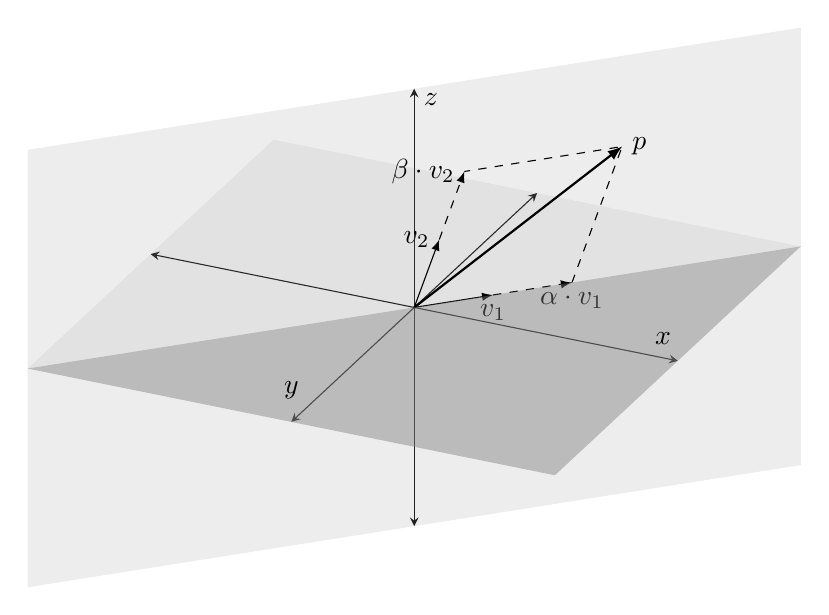
\begin{tikzpicture}
            \begin{axis}[width=11.4cm,height=11.4cm,
            xlabel=$x$, ylabel=\empty, zlabel=$z$,
            xmin=-4.9, xmax=4.9,
            ymin=-4.9, ymax=4.9,
            zmin=-4.9, zmax=4.9,
            axis lines=center,
            %xticklabel=\empty,
            %yticklabel=\empty,
            %zticklabel=\empty,
            axis line style={stealth-stealth},
            ticks=none,
            ]
                \fill[gray,opacity=0.1] (xyz cs:x=-4.9,y=-4.9,z=0) -- (xyz cs:x=4.9,y=-4.9,z=0) -- (xyz cs:x=4.9,y=4.9,z=0) --  (xyz cs:x=-4.9,y=4.9,z=0) -- cycle;
                \fill[gray!70,opacity=0.2] (xyz cs:x=-4.9,y=-4.9,z=-4.9) -- (xyz cs:x=4.9,y=4.9,z=-4.9) -- (xyz cs:x=4.9,y=4.9,z=4.9) --  (xyz cs:x=-4.9,y=-4.9,z=4.9) -- cycle;
                
                \draw[dash pattern=on 3pt off 3pt] (2,2,0) -- (2,4,2) -- (0,2,2);
                
                \draw[-latex,dash pattern=on 3pt off 3pt] (1,1,0) -- (2,2,0) node[below] {$\alpha \cdot \mathbb{v}_1$};
                \draw[-latex] (0,0,0) -- (1,1,0) node[below]{$ \mathbb{v}_1$};

                \draw[-latex,dash pattern=on 3pt off 3pt] (0,1,1) -- (0,2,2) node[left] {$\beta \cdot \mathbb{v}_2$};
                \draw[-latex] (0,0,0) -- (0,1,1) node[left]{$\mathbb{v}_2$};

                \draw[-latex,thick] (0,0,0) -- (2,4,2) node[right]{$\mathbb{p}$};

                %\node [inner sep=2pt,outer sep=0pt] (O) at (axis cs:0,0,0) {};
                %\node [align=center] (origin) at ([xshift=1.5cm,yshift=-1.3cm]O) {$\mathbb{0}$};
                %\draw [shorten <=.1cm,stealth-] (O) to [out=-30,in=160] (origin.west);
                
                \fill[gray,opacity=0.4] (xyz cs:x=-4.9,y=-4.9,z=0) -- (xyz cs:x=4.9,y=-4.9,z=0) -- (xyz cs:x=4.9,y=4.9,z=0) -- cycle;
                \node at (0,-4.9,0.7) {$y$};
            \end{axis}
        \end{tikzpicture}
        \caption{Representación del plano $x - y + z = 0$}
    \end{figure}
\end{example}

\section{Dependencia e independencia lineal}

\begin{definition}
    Sea $V$ un espacio vectorial sobre $K$ y sean $\mathbb{v}_1$, $\mathbb{v}_2$, $\dots$, $\mathbb{v}_n$ vectores en $V$. Se dice que los vectores $\mathbb{v}_1$, $\mathbb{v}_2$, $\dots$, $\mathbb{v}_n$ son linealmente dependientes (l.d), si existen $a_1$, $a_2$, $\dots$, $a_n \in K$ no todos $0$ tales que
    $$a_1 \mathbb{v}_1 + a_2 \mathbb{v}_2 + \cdots + a_n \mathbb{v}_n = \mathbb{0}$$
    En caso contrario, se les llama linealmente independientes (l.i).
\end{definition}

\begin{example}
    En $\RR[2]$, verifique que $\displaystyle \mathbb{v}_1 = \binom{1}{3}$ y $\displaystyle \mathbb{v}_1 = \binom{2}{6}$ son linealmente dependientes. \\
    \solucion Sean $a_1 = 1$ y $\displaystyle a_2 = -\frac{1}{2}$, tenemos\sideFigure[\label{HAHAHAVVAGAGHRRQ}]{
    \begin{center}
        \begin{tikzpicture}
            \draw[thick,-Stealth] (-1,0) -- (4,0) node[below left] {$x$};
            \draw[thick,-Stealth] (0,-1) -- (0,7) node[below left] {$y$};
            \draw[dash pattern=on 3pt off 3pt] (0,3) node[left] {$3$} -- (1,3) -- (1,0) node[below] {$1$};
            \draw[dash pattern=on 3pt off 3pt] (0,6) node[left] {$6$} -- (2,6) -- (2,0) node[below] {$2$};
            \draw[-latex] (0,0) -- (2,6) node [right] {$\mathbb{v}_2$};
            \draw[-latex] (0,0) -- (1,3) node [right] {$\mathbb{v}_1$};
        \end{tikzpicture}
    \end{center}
    }
    \begin{align*}
        a_1\mathbb{v}_1 + a_2\mathbb{v}_2 & = 1 \cdot \binom{1}{3} + \left( -\frac{1}{2} \right) \cdot \binom{2}{6} \\
        & = \binom{1}{3} + \binom{-1}{-3} && \text{por def. de producto escalar} \\
        & = \binom{1+(-1)}{3+(-3)} && \text{por def. de suma en } \RR[2] \\
        & = \binom{0}{0} \\
        & = \mathbb{0}
    \end{align*}
    Además, observemos que
    $$\binom{2}{6} = 2 \cdot \binom{1}{3}$$
    Geométricamente tenemos la figura \ref{HAHAHAVVAGAGHRRQ}.
\end{example}

\begin{theorem}
    Dos vectores en un espacio vectorial son linealmente dependientes si y solo si uno de ellos es un múltiplo escalar del otro. \\
    \demostracion Se deja como ejercicio al lector.
\end{theorem}

\begin{example}
    Verifique que en $\RR[3]$ los vectores $\displaystyle \mathbb{v}_1 = \begin{pmatrix*}[r] 1 \\ -3 \\ 0 \end{pmatrix*}$, $\displaystyle \mathbb{v}_2 = \begin{pmatrix} 3 \\ 0 \\ 4 \end{pmatrix}$ y $\displaystyle \mathbb{v}_3 = \begin{pmatrix} 11 \\ -6 \\ 12 \end{pmatrix}$ son linealmente dependientes. \\
    \solucion Hay que demostrar que existen $a_1$, $a_2$, $a_3 \in \RR$ no todos cero, tales que
    $$a_1\mathbb{v}_1 + a_2\mathbb{v}_2 + a_3\mathbb{v}_3 = \mathbb{0}$$
    esto es
    \begin{equation}
        a_1 \cdot \begin{pmatrix*}[r] 1 \\ -3 \\ 0 \end{pmatrix*} + a_2 \cdot \begin{pmatrix} 3 \\ 0 \\ 4 \end{pmatrix} + a_3 \cdot \begin{pmatrix} 11 \\ -6 \\ 12 \end{pmatrix} = \begin{pmatrix} 0 \\ 0 \\ 0 \end{pmatrix} \label{ec22}
    \end{equation}
    Veamos que uno de los vectores se puede expresar como combinación lineal de los otros dos, es decir
    $$\begin{pmatrix} 11 \\ -6 \\ 12 \end{pmatrix} = a_1 \cdot \begin{pmatrix*}[r] 1 \\ -3 \\ 0 \end{pmatrix*} + a_2 \cdot \begin{pmatrix} 3 \\ 0 \\ 4 \end{pmatrix}$$
    Con $a_1 = 2$, $a_2 = 3$ y $a_3 = -1$, de la ecuación \eqref{ec22}
    \begin{align*}
        2 \cdot \begin{pmatrix*}[r] 1 \\ -3 \\ 0 \end{pmatrix*} + 3 \cdot \begin{pmatrix} 3 \\ 0 \\ 4 \end{pmatrix} - 1 \cdot \begin{pmatrix*}[r] 11 \\ -6 \\ 12 \end{pmatrix*} & = \begin{pmatrix*}[r] 2 \\ -6 \\ 0 \end{pmatrix*} + \begin{pmatrix} 9 \\ 0 \\ 12 \end{pmatrix} + \begin{pmatrix*}[r] -11 \\ 6 \\ -12 \end{pmatrix*} \\
        & = \begin{pmatrix} 2+9-11 \\ -6+0+6 \\ 0+12-12 \end{pmatrix} \\
        & = \begin{pmatrix} 0 \\ 0 \\ 0 \end{pmatrix} = \mathbb{0}
    \end{align*}
    Por tanto, $\mathbb{v}_1$, $\mathbb{v}_2$ y $\mathbb{v}_3$ son vectores linealmente dependientes.
\end{example}

\begin{example}
    Verifique que los vectores $\displaystyle e_1 = \binom{1}{0}$ y $\displaystyle e_2 = \binom{0}{1}$ son linealmente independientes en $\RR[2]$. \\
    \solucion Supongamos que son linealmente dependientes, entonces existen $a_1$, $a_2 \in \RR$ no todos ceros tales que $a_1e_1 + a_2e_2 = \mathbb{0}$. Luego
    \begin{align*}
        \mathbb{0} & = a \cdot \binom{1}{0} + a_2 \cdot \binom{0}{1} \\
        & = \binom{a_1}{0} + \binom{0}{a_2} \\
        & = \binom{a_1}{a_2}
    \end{align*}
    Por tanto, $a_1 = 0$ y $a_2 = 0$, entonces el supuesto es falso y se cumple lo contrario, esto es que $e_1$ y $e_2$ son linealmente independientes.
\end{example}

\begin{example}
    En $\RR[n]$, sean $\displaystyle e_1 = \left( \begin{array}{c} 1 \\ 0 \\ 0 \\ \vdots \\ 0 \\ 0 \end{array} \right)$, $\displaystyle e_2 = \left( \begin{array}{c} 0 \\ 1 \\ 0 \\ \vdots \\ 0 \\ 0 \end{array} \right)$, $\dots$, $\displaystyle e_n = \left( \begin{array}{c} 0 \\ 0 \\ 0 \\ \vdots \\ 0 \\ 1 \end{array} \right)$ son linealmente independientes en $\RR[n]$. \\
    \solucion Se deja como ejercicio al lector probar que dichos vectores son l.i.
\end{example}

\begin{theorem}
    $\RR[n]$ como espacio vectorial sobre $\RR$, tiene a los más $n$ vectores linealmente independientes.
\end{theorem}

\begin{example}
    Considere el espacio vectorial $P_n(x)$ sobre $\RR$. Determine tres vectores en $P_2(x)$ que sean linealmente independientes. \\
    \solucion $\left\{ 1, x, x^2 \right\}$ es l.i, empleando la definición:
    \begin{equation}
        a_1 \cdot 1 + a_2 \cdot x + a_3 \cdot x^2 = \mathbb{0} \label{ec23}
    \end{equation}
    hay que demostrar que $a_1$, $a_2$ y $a_3$ son $0$. De la ecuación \eqref{ec23}
    $$a_1 \cdot 1 + a_2 \cdot x + a_3 \cdot x^2 = 0 \cdot 1 + a \cdot x + 0 \cdot x^2$$
    si y solo si los respectivos coeficientes son iguales, entonces $a_1 = 0$, $a_2 = 0$, $a_3 = 0$. Por lo tanto, $\left\{ 1, x, x^2 \right\}$ es l.i. Determinemos otros tres vectores l.i, sean $\mathbb{v}_1 = 1$, $\mathbb{v}_2 = 1+x$, $\mathbb{v}_3 = 1+x+x^2 \in P_2(x)$. Veamos que son l.i, por la definición sea
    \begin{equation}
        a_1\mathbb{v}_1 + a_2\mathbb{v}_2 + a_3\mathbb{v}_3 = \mathbb{0} \label{ec24}
    \end{equation}
    hay que demostrar que $a_1 = 0$, $a_2 = 0$ y $a_3 = 0$. De la ecuación \eqref{ec24},
    \begin{align*}
        0 \cdot 1 + 0 \cdot x + 0 \cdot x^2 & = a_1 \cdot 1 + a_2 \cdot (1+x) + a_3 \cdot \left( 1+x+x^2 \right) \\
        & = a_1 + (a_2 \cdot 1 + a_2 \cdot x) + \left( a_3 \cdot 1 + a_3 \cdot x + a_3 \cdot x^2 \right) \\
        & = a_1 + a_2 + a_3 + a_2 \cdot x + a_3 \cdot x + a_3 \cdot x^2 \\
        & = (a_1 + a_2 + a_3) + (a_2 + a_3) \cdot x + a_3 \cdot x^2
    \end{align*}
    si y solo si
    \begin{align*}
        a_1 + a_2 + a_3 & = 0 \\
        a_2 + a_3 & = 0 \\
        a_3 & = 0
    \end{align*}
    de donde se sigue que $a_1 = 0$, $a_2 = 0$ y $a_3 = 0$. Por tanto, $\left\{ 1, 1+x, 1+x^2 \right\}$ es l.i.
\end{example}

\section{Base y dimensión}

\begin{definition}
    Sea $V$ un espacio vectorial sobre $K$ y sean $\mathbb{v}_1$, $\mathbb{v}_2$, $\dots$, $\mathbb{v}_n \in V$. Decimos que $\left\{ \mathbb{v}_1, \mathbb{v}_2, \dots, \mathbb{v}_n \right\}$ es una \textbf{base} de $V$ si:
    \begin{enumerate}[label=\roman*)]
        \item $\mathbb{v}_1$, $\mathbb{v}_2$, $\dots$, $\mathbb{v}_n$ son l.i
        \item $V = \Gen \left( \{ \mathbb{v}_1, \mathbb{v}_2, \dots, \mathbb{v}_n \} \right)$
    \end{enumerate}
\end{definition}

\begin{examples}~
    \begin{enumerate}
        \item En $P_n(x)$, $\left\{ 1, x, x^2, \dots, x^n \right\}$ forman una base para $P_n(x)$.
        \item En $\RR[2]$, $\displaystyle e_1 = \binom{1}{0}$ y $\displaystyle e_2 = \binom{0}{1}$ forman una base en $\RR[2]$, pues son l.i y generan a $\RR[2]$.
        \item Para $\RR[n]$, $\displaystyle e_1 = \left( \begin{array}{c} 1 \\ 0 \\ 0 \\ \vdots \\ 0 \\ 0 \end{array} \right)$, $\displaystyle e_2 = \left( \begin{array}{c} 0 \\ 1 \\ 0 \\ \vdots \\ 0 \\ 0 \end{array} \right)$, $\dots$, $\displaystyle e_n = \left( \begin{array}{c} 0 \\ 0 \\ 0 \\ \vdots \\ 0 \\ 1 \end{array} \right)$ forman una base en $\RR[n]$, donde $\{ e_1, e_2, \dots, e_n \}$ se le llama la base canónica de $\RR[n]$.
    \end{enumerate}
\end{examples}

\begin{remark}
    Recordemos que si $A$ es un conjunto no vacío, se define la cardinalidad del conjunto $A$, denotado por $|A|$, como el número de elementos de $A$. Además, se dice que el conjunto $A$ es finito si $|A| < \infty$. En caso contrario, se dice que el conjunto es infinito. Por ejemplo, el conjunto $\NN$.
\end{remark}

\begin{definition}
    Sea $V$ un espacio vectorial sobre $K$. Se llama dimensión del espacio vectorial $V$, a la cardinalidad de la base de $V$, y se denotará por $\Dim V$.
\end{definition}

\begin{examples}~
    \begin{enumerate}
        \item En $P_n(x)$, una base de $P_n(x)$ es $\mathcal{P} = \left\{ 1, x, x^2, \dots, x^n \right\}$. Entonces $\Dim P_n(x) = |\mathcal{P}| = n+1$.
        \item En $\RR[2]$, una base de $\RR[2]$ es $\displaystyle \mathcal{A} = \left\{ \binom{1}{0},  \binom{0}{1} \right\}$. Entonces $\Dim \RR[2] = |\mathcal{A}| = 2$.
        \item En $\RR[n]$, una base de $\RR[n]$ es $\displaystyle \mathcal{B} = \left\{ \left( \begin{array}{c} 1 \\ 0 \\ 0 \\ \vdots \\ 0 \\ 0 \end{array} \right),  \left( \begin{array}{c} 0 \\ 1 \\ 0 \\ \vdots \\ 0 \\ 0 \end{array} \right),  \dots,  \left( \begin{array}{c} 0 \\ 0 \\ 0 \\ \vdots \\ 0 \\ 1 \end{array} \right) \right\}$. Entonces $\Dim \RR[n] = |\mathcal{B}| = n$.
    \end{enumerate}
\end{examples}

\begin{remark}
    Dado el espacio vectorial $V = \left\{ f: \RR \longrightarrow \RR \mid f \text{ es continua} \right\}$, es un espacio vectorial sobre $\RR$ y $\Dim V = \infty$.
\end{remark}

\begin{theorem}
    Sea $V$ un espacio vectorial y $\mathcal{B} = \{ \mathbb{v}_1,  \mathbb{v}_2,  \dots,  \mathbb{v}_n \}$ base de $V$. Entonces todo elemento de $V$ se expresa de manera única a partir de los elementos de la base. Es decir, dado $\mathbb{u} \in V$, existen $a_1$, $a_2$, $\dots$, $a_n \in K$ únicos tales que
    \begin{equation}
        \mathbb{u} = a_1\mathbb{v}_1 + a_2\mathbb{v}_2 + \cdots + a_n\mathbb{v}_n \label{ec25}
    \end{equation}
    \demostracion Supongamos que existen $b_1$, $b_2$, $\dots$, $b_n \in K$ tales que
    \begin{equation}
        \mathbb{u} = b_1\mathbb{v}_1 + b_2\mathbb{v}_2 + \cdots + b_n\mathbb{v}_n \label{ec26}
    \end{equation}
    Se demostrará que $a_i = b_i$, para $i = 1$, $2$, $\dots$, $n$. Sea
    \begin{align*}
        -\mathbb{u} & = (-1) \cdot \mathbb{u} \\
        & = (-1) \cdot (b_1\mathbb{v}_1 + b_2\mathbb{v}_2 + \cdots + b_n\mathbb{v}_n) \\
        & = (-1)b_1\mathbb{v}_1 + (-1)b_2\mathbb{v}_2 + \cdots + (-1)b_n\mathbb{v}_n \\
        & = (-b_1)\mathbb{v}_1 + (-b_2)\mathbb{v}_2 + \cdots + (-b_n)\mathbb{v}_n
    \end{align*}
    Ahora, de las expresiones \eqref{ec25} y \eqref{ec26} tenemos
    \begin{align*}
        \mathbb{0} & = \mathbb{u} + (-\mathbb{u}) \\
        & = a_1\mathbb{v}_1 + a_2\mathbb{v}_2 + \cdots + a_n\mathbb{v}_n + (-b_1)\mathbb{v}_1 + (-b_2)\mathbb{v}_2 + \cdots + (-b_n)\mathbb{v}_n \\
        & = \big(a_1+(-b_1)\big)\mathbb{v}_1 + \big(a_2+(-b_2)\big)\mathbb{v}_2 + \cdots + \big(a_n+(-b_n)\big)\mathbb{v}_n
    \end{align*}
    Entonces $\big(a_1+(-b_1)\big) = 0$, $\big(a_2+(-b_2)\big) = 0$, $\dots$, $\big(a_n+(-b_n)\big) = 0$, ya que $\mathbb{v}_1$, $\mathbb{v}_2$, $\dots$, $\mathbb{v}_n$ son l.i, se sigue que $b_1 = a_1$, $b_2 = a_2$, $\dots$, $b_n = a_n$. Por lo tanto, $\mathbb{u}$ se expresa de manera única.
\end{theorem}

\begin{theorem}
    Sea $V$ un espacio vectorial de dimensión finita $n$, sobre un campo $K$. Entonces dados $\mathbb{v}_1$, $\mathbb{v}_2$, $\dots$, $\mathbb{v}_m \in V$ linealmente independientes, se cumple que $m \leq n$.
\end{theorem}

\begin{remark}
    A los subesapacios distintos a $V$ y $\{ \mathbb{0} \}$ se les llama subespacios propios.
\end{remark}

\begin{observation}
    Todo espacio vectorial admite una base (lema de Zorn).\\
    \demostracion Puede verse una demostración en: Dugundji, James; TOPOLOGY. Allyn and Bacon, Inc. 1975
\end{observation}

\begin{theorem}\label{theorem:teorema1.5.1}
    Sea $V$ un espacio vectorial sobre $K$ con dimension finita $n$, y sea $H \subseteq V$ un subespacio, entonces $\Dim H \leq \Dim V$. \\
    \demostracion Sea $\{ \mathbb{h}_1,  \mathbb{h}_2,  \dots,  \mathbb{h}_k \} \subseteq H$ una base de $H$. Al ser una base, entonces $\mathbb{h}_1$, $\mathbb{h}_2$, $\dots$, $\mathbb{h}_k$ son l.i. Por el teorema anterior, $k \leq n$, de donde se sigue que
    $$\Dim H = k \leq n = \Dim V$$
    Por tanto, $\Dim H \leq \Dim V$.
\end{theorem}

\begin{example}
    Sea $V = \RR[2]$ y sea
    $$\displaystyle H = \left\{ \binom{x}{x} \in \RR[2] \mid x \in \RR \right\}$$
    Sabemos que $H$ es una recta que pasa por $\displaystyle \binom{0}{0}$ y que además $\Dim \RR[2] = 2$. Ahora
    \begin{align*}
        H & = \left\{ \binom{x}{x} \mid x \in \RR \right\} \\
        & = \left\{ x \cdot \binom{1}{1},  x \in \RR \right\}
    \end{align*}
    Esto es
    $$x \cdot \mathbb{h} \text{ con } x \in \RR \quad \text{ y } \quad \mathbb{h} = \binom{1}{1}$$
     Geométricamente tenemos la figura \ref{UABABJABBVAJAHA}. Entonces\sideFigure[\label{UABABJABBVAJAHA}]{
     \begin{tikzpicture}
        \draw[thick,-Stealth] (-1,0) -- (4,0) node[below left] {$x$};
        \draw[thick,-Stealth] (0,-1) -- (0,4) node[below left] {$y$};
        \draw[dash pattern=on 3pt off 3pt] (1,1) -- (3,3) node [above right] {$H$};
        \draw[-latex] (0,0) -- (1,1) node[below right] {$\mathbb{h}$};
        \draw[dash pattern=on 3pt off 3pt] (0,0) -- (-1,-1);
    \end{tikzpicture}
    }
    \begin{align*}
        H & = \left\{ x \cdot \binom{1}{1},  x \in \RR \right\} \\
        & = \Gen \left( \left\{ \binom{1}{1} \right\} \right)
    \end{align*}
    Así $H$ es generado por $\displaystyle \mathbb{h} = \binom{1}{1}$ y además es l.i. Entonces $\displaystyle \left\{ \binom{1}{1} \right\}$ es una base de $H$. Se sigue que $\Dim H = 1$ y $1 \leq 2$, por lo que
    $$\Dim H = 1 \leq 2 = \Dim \RR[2]$$
\end{example}

\begin{theorem}\label{def:n_vectores_base}
    Sea $V$ un espacio vectorial sobre $K$ de dimensión finita $n$, entonces cualquier conjunto de vectores $\mathbb{v}_1$, $\mathbb{v}_2$, $\dots$, $\mathbb{v}_n$ linealmente independientes constituyen una base de $V$. \\
    \demostracion Por hipótesis, tenemos que $\mathbb{v}_1$, $\mathbb{v}_2$, $\dots$, $\mathbb{v}_n$ son l.i. Para demostrar que $\{ \mathbb{v}_1, \mathbb{v}_2, \dots, \mathbb{v}_n \}$ genera a $V$ supongamos lo contrario, esto es que $\{ \mathbb{v}_1, \mathbb{v}_2, \dots, \mathbb{v}_n \}$ no genera a $V$. Entonces existe un $\mathbb{u} \in V$ tal que
    $$\mathbb{u} \notin \Gen(\{ \mathbb{v}_1, \mathbb{v}_2, \dots, \mathbb{v}_n \})$$
    Afirmamos que $\mathbb{u}$ es l.i con $\mathbb{v}_1$, $\mathbb{v}_2$, $\dots$, $\mathbb{v}_n$, es decir, $\mathbb{v}_1$, $\mathbb{v}_2$, $\dots$, $\mathbb{v}_n$, $\mathbb{u}$ son l.i. Así dada la combinación lineal
    \begin{equation}
        a_1\mathbb{v}_1 + a_2\mathbb{v}_2 + \cdots + a_n\mathbb{v}_n + b\mathbb{u} = \mathbb{0} \label{ec27}
    \end{equation}
    Afirmamos que $b = 0$. Supongamos lo contrario, es decir, $b \neq 0$. De la ecuación \eqref{ec27},
    $$a_1\mathbb{v}_1 + a_2\mathbb{v}_2 + \cdots + a_n\mathbb{v}_n + \mathbb{0} = \mathbb{0} + (-b\mathbb{u})$$
    Multiplicando por el inverso multiplicativo de $-b \in K$, es decir, $\displaystyle (-b)^{-1} = - \frac{1}{b}$, obtenemos
    $$\left(-\frac{a_1}{b}\right)\mathbb{v}_1 + \left(-\frac{a_2}{b}\right)\mathbb{v}_2 + \cdots + \left(-\frac{a_n}{b}\right)\mathbb{v}_n = \mathbb{u} \in \Gen(\{ \mathbb{v}_1, \mathbb{v}_2, \dots, \mathbb{v}_n \})$$
    lo cual es una contradicción, pues $\mathbb{u} \notin \Gen(\{ \mathbb{v}_1, \mathbb{v}_2, \dots, \mathbb{v}_n \})$. Por lo tanto, $b = 0$. Sustituyendo en la ecuación \eqref{ec27}
    $$a_1\mathbb{v}_1 + a_2\mathbb{v}_2 + \cdots + a_n\mathbb{v}_n + 0 \cdot \mathbb{u} = \mathbb{0}$$
    Así
    $$a_1\mathbb{v}_1 + a_2\mathbb{v}_2 + \cdots + a_n\mathbb{v}_n = \mathbb{0}$$
    Entonces
    $$a_1 = a_2 = \cdots = a_n = 0$$
    ya que $\mathbb{v}_1$, $\mathbb{v}_2$, $\dots$, $\mathbb{v}_n$ son l.i. Por el teorema \ref{theorem:teorema1.5.1},
    $$n + 1 \leq \Dim V = n$$
    lo cual es una contradicción. Por lo tanto $\{ \mathbb{v}_1,  \mathbb{v}_2,  \dots,  \mathbb{v}_n \}$ genera a $V$.
\end{theorem}

\begin{example}
    Sabemos que la dimensión de $P_2(x) = 3$. Entonces el conjunto $\left\{ 1-x^2,  x \right\}$ no puede ser una base de $P_2(x)$, pues tendríamos a lo más dos vectores linealmente independientes y $2 < 3 = \Dim P_2(x)$. Por tanto, por el teorema anterior $\left\{ 1-x^2,  x \right\}$ no es una base de $P_2(x)$.
\end{example}

\begin{theorem}
    Si $\left\{ \mathbb{u}_1, \mathbb{u}_2, \dots, \mathbb{u}_m \right\}$ y $\left\{ \mathbb{v}_1, \mathbb{v}_2, \dots, \mathbb{v}_n \right\}$ son dos bases de un espacio vectorial $V$ de dimensión finita, entonces $m = n$. Es decir, cualesquiera dos bases de un espacio vectorial $V$ de dimensión finita tienen el mismo número de vectores. \\
    \demostracion Sea $S_1 = \left\{ \mathbb{u}_1, \mathbb{u}_2, \dots, \mathbb{u}_m \right\}$ y $S_2 = \left\{ \mathbb{v}_1, \mathbb{v}_2, \dots, \mathbb{v}_n \right\}$ dos bases de $V$. Es necesario demostrar que $m = n$. Para ello, se procede a mostrar que si $m > n$, entonces $S_1$ es linealmente independiente, lo cual contradice la premisa de que $S_1$ es una base. Esto establecerá que $m \leq n$. De manera análoga, se demuestra que $n \leq m$, lo que concluye el teorema. Por lo tanto, es suficiente demostrar que si $m > n$, entonces $S_1$ es un conjunto linealmente dependiente. Dado que $S_2$ es una base, cada vector $\mathbb{u}_i$ puede expresarse como una combinación lineal de los vectores $\mathbb{v}_j$. Por consiguiente, se tiene
    \begin{equation}
        \begin{aligned}
           \mathbb{u}_1 & = a_{11} \mathbb{v}_1 + a_{12} \mathbb{v}_2 + \cdots + a_{1n} \mathbb{v}_n \\
            \mathbb{u}_2 & = a_{21} \mathbb{v}_1 + a_{22} \mathbb{v}_2 + \cdots + a_{2n} \mathbb{v}_n \\
            & \vdots \\
            \mathbb{u}_m & = a_{m1} \mathbb{v}_1 + a_{m2} \mathbb{v}_2 + \cdots + a_{mn} \mathbb{v}_n
        \end{aligned} \label{ECUACION5.5.1}
    \end{equation}
    Para demostrar que $S_1$ es linealmente dependiente, se deben encontrar escalares $c_1$, $c_2$, $\dots$, $c_m$ no todos cero, tales que
    \begin{equation}
        c_1\mathbb{u}_1 + c_2\mathbb{u}_2 + \cdots + c_m\mathbb{u}_m = \mathbb{0} \label{ECUACION5.5.2}
    \end{equation}
    Sustituyendo \eqref{ECUACION5.5.1} en \eqref{ECUACION5.5.2} se obtiene
    $$c_1\left( a_{11} \mathbb{v}_1 + a_{12} \mathbb{v}_2 + \cdots + a_{1n} \mathbb{v}_n \right) + c_2\left( a_{21} \mathbb{v}_1 + a_{22} \mathbb{v}_2 + \cdots + a_{2n} \mathbb{v}_n \right) + \cdots + c_m\left( a_{m1} \mathbb{v}_1 + a_{m2} \mathbb{v}_2 + \cdots + a_{mn} \mathbb{v}_n \right) = \mathbb{0}$$
    Es decir,
    $$\left( a_{11}c_1 + a_{21}c_2 + \cdots + a_{m1}c_m \right)\mathbb{v}_1 + \left( a_{12}c_1 + a_{22}c_2 + \cdots + a_{m2}c_m \right)\mathbb{v}_2 + \cdots + \left( a_{1n}c_1 + a_{2n}c_2 + \cdots + a_{mn}c_m \right)\mathbb{v}_m = \mathbb{0}$$
    Pero $\mathbb{v}_1$, $\mathbb{v}_2$, $\dots$, $\mathbb{v}_n$ son linealmente independientes, entonces
    \begin{align*}
        a_{11}c_1 + a_{21}c_2 + \cdots + a_{m1}c_m & = 0 \\
        a_{12}c_1 + a_{22}c_2 + \cdots + a_{m2}c_m & = 0 \\
        & \vdots \\
        a_{1n}c_1 + a_{2n}c_2 + \cdots + a_{mn}c_m & = 0
    \end{align*}
    Nótese que el sistema anterior constituye un sistema de $n$ ecuaciones con $m$ incógnitas, lo que implica que $m > n$. Por lo tanto, el sistema tiene un número infinito de soluciones. De esta manera, existen escalares $c_1$, $c_2$, $\dots$, $c_m$, no todos nulos, tales que la ecuación \eqref{ECUACION5.5.2} se satisface, lo que implica que $S_1$ es un conjunto linealmente dependiente. Esta contradicción demuestra que $m \leq n$. Al intercambiar los roles de $S_1$ y $S_2$, se demuestra que $n \leq m$, lo que completa la prueba.
\end{theorem}

\begin{adjustwidth}{-2.15cm}{-\wholeMargin -3.5cm}
    \begin{tcolorbox}[
        theorem style=change break,
        enhanced,
        breakable,
        boxrule=0pt,
        frame hidden,
        left = 2cm,
        right = 2cm,
        top=6mm,
        bottom=1mm,
        colback=gray!20,
        coltitle=black,
        attach title to upper={\ },
        sharp corners,
        title = Algunas observaciones:,
        fonttitle=\bfseries\LARGE,
        fontupper=\normalsize
    ]
        \begin{tikzpicture}[remember picture,overlay] \filldraw[gray!20] (current page.south west) rectangle ($(current page.south east) + (0,3)$); \end{tikzpicture}
        \begin{multicols}{2}
            \hspace*{5.5mm}En este capítulo hemos explorado los fundamentos de los espacios vectoriales reales. Es importante destacar que nos hemos enfocado exclusivamente en el estudio de vectores y operaciones definidas sobre ellos en el contexto de números reales. Sin embargo, es crucial reconocer que todo lo que hemos aprendido en este capítulo se puede generalizar y extender al ámbito de los espacios vectoriales complejos. A medida que avanzamos hacia el capítulo \ref{chap:espacios_complejos}, exploraremos cómo los números complejos enriquecen nuestra comprensión de los espacios vectoriales y amplían nuestras capacidades de modelado y resolución de problemas.
            
            \hspace*{5.5mm}Es importante destacar que $\CC[n]$, el espacio de los vectores $n$-dimensionales con coeficientes complejos, constituye un espacio vectorial sobre los números complejos $\CC$. Demostraremos en el capítulo \ref{chap:espacios_complejos} que las propiedades fundamentales de los espacios vectoriales se mantienen cuando trabajamos con coeficientes complejos. Así, aunque nos hemos centrado en los espacios vectoriales reales en este capítulo, es importante reconocer la relevancia y la conexión entre ambos ámbitos. La extensión de nuestros conocimientos a los espacios vectoriales complejos nos permitirá abordar una gama aún más amplia de problemas y aplicaciones en matemáticas y disciplinas relacionadas.
            
            \hspace*{5.5mm}Para aquellos lectores que no estén familiarizados con los números complejos, se recomienda consultar el \hyperref[chap:numeros-complejos]{Apéndice B}, donde se proporciona una introducción detallada y accesible a este campo. En este apéndice, se abordan los conceptos básicos de los números complejos, incluyendo operaciones fundamentales como la suma, la resta, la multiplicación y la división; así como propiedades importantes como el conjugado y el módulo.
        \end{multicols}
    \end{tcolorbox}
\end{adjustwidth}

\newpage

\section{Ejercicios}

\noindent
De los problemas 1 al 15 determine si el conjunto dado es un espacio vectorial. De no ser así proporcione una lista de los axiomas que no se cumplen.
\begin{enumerate}
    \item El conjunto de números naturales $\NN$ como vectores, el conjunto de números naturales $\NN$ como escalares y la operación de multiplicación para números naturales.
    \item El conjunto de números naturales $\NN$ como vectores, el conjunto de números naturales $\NN$ como escalares, la operación de suma para números naturales y la multiplicación entre números naturales para la operación de multiplicación de escalar y vector.
    \item El conjunto de números enteros $\ZZ$ como vectores, el conjunto de números naturales $\NN$ como escalares, la operación de suma para números enteros y la multiplicación entre números enteros para la operación de multiplicación de escalar y vector.
    \item $\left\{ \begin{pmatrix} x \\ y \end{pmatrix} \mid y \leq 0 \text{ donde } x, y \in \RR \right\}$ con la suma de vectores y multiplicación por un escalar usuales.
    \item Los vectores en el plano que está en el primer cuadrante.
    \item El conjunto de vectores en $\RR[2]$ de la forma $\begin{pmatrix} x \\ x \end{pmatrix}$.
    \item El conjunto de vectores los números racionales $\QQ$ con la operación de suma, el conjunto de escalares los números enteros $\ZZ$ y la operación de multiplicación de escalar y vector la multiplicación usual.
    \item El conjunto de polinomios de grado menor o igual a $n$ con término constante cero.
    \item El conjunto de polinomios de grado menor o igual a $n$ con término constante $a_{0}$ positivo.
    \item El conjunto de polinomios de grado menor o igual a $n$ con término constante $a_{0}$ negativo.
    \item El conjunto de funciones continuas de valores reales definidas en $[0, 1]$ con $f(0) = 0$ y $f(1) = 0$ bajo las operaciones del ejemplo \ref{ejemplo5.1.8}.
    \item El conjunto de puntos en $\RR[3]$ que se encuentran sobre una recta que pasa por el origen.
    \item El conjunto de puntos en $\RR[3]$ que se encuentran sobre la recta $x = t+1$, $y = 2t$, $z = t-1$.
    \item El conjunto de funciones diferenciables definidas en $[0, 1]$ con las operaciones del ejemplo \ref{ejemplo5.1.8}.
    \item El conjunto de números reales de la forma $a+b \sqrt{2}$, donde $a$ y $b$ son números racionales, bajo la suma de números reales usual y la multiplicación por un escalar definida sólo para escalares racionales.
\end{enumerate}
De los problemas 16 al 34 determine si el subconjunto dado $H$ del espacio vectorial $V$ es un subespacio de $V$.
\begin{enumerate}[resume]
    \item $V=\RR[2]$; $H=\left\{ \begin{pmatrix} x \\ y \end{pmatrix} \mid x=3, y \in \RR \right\}$
    \item $V=\RR[2]$; $H=\left\{ \begin{pmatrix} x \\ y \end{pmatrix} \mid y \geq 0 \right\}$\newpage
    \item $V=\RR[2]$; $H=\left\{ \begin{pmatrix} x \\ y \end{pmatrix} \mid x=y \right\}$
    \item $V=\RR[2]$; $H=\left\{ \begin{pmatrix} x \\ y \end{pmatrix} \mid y=2 x \right\}$
    \item $V=\RR[3]$; $H = \operatorname{el~plano} x y$
    \item $V=\RR[2]$; $H=\left\{ \begin{pmatrix} x \\ y \end{pmatrix} \mid x^{2}+y^{2} \leq 1\right\}$
    \item $V=\RR[2]$; $H=\left\{ \begin{pmatrix} x \\ y \end{pmatrix} \mid x^{2}+y^{3}<1\right\}$
    \item $V=\RR$; $H=\QQ$
    \item $V=P_{n}$; $H=\left\{p \in P_{n}\mid p(0)=0\right.$ y $\left.p^{\prime}(0)=0\right\}$
    \item $V=P_{4}$; $H=\left\{p \in P_{4}\mid p(0)=0\right\}$
    \item $V=P_{n}$; $H=\left\{p \in P_{n}\mid p(0)=0\right\}$
    \item $V=P_{n}$; $H=\left\{p \in P_{n}\mid p(0)=1\right\}$
    \item $V=C[0,1]$; $H=\{f \in C[0,1]\mid f(0)=f(1)=0\}$
    \item $V=C[0,1]$; $H=\{f \in C[0,1]\mid f(0)=2\}$
    \item $V=C^{1}[0,1]$; $H=\left\{f \in C^{1}[0,1]\mid f^{\prime}(0)=0\right\}$
    \item $V=C[a, b]$; donde $a$, $b \in \RR$ y $a<b$; $\displaystyle H=\left\{f \in C[a, b]\mid \int_{a}^{b} f(x) d x=0\right\}$
    \item $V=C[a, b]$; $\displaystyle H=\left\{f \in C[a, b]\mid \int_{a}^{b} f(x) d x=1\right\}$
    \item $V=C[a, b]$; $\displaystyle H=\left\{f \in C[a, b]\mid \int_{a}^{b} f^{2}(x) d x=0\right\}$
    \item Sea $H=\left\{ \begin{pmatrix} x \\ y \\ z \\ w \end{pmatrix} \mid a x+b y+c z+d w=0\right\}$, donde $a, b, c$ y $d$ son números reales, no todos cero. Demuestre que $H$ es un subespacio propio de $\RR[4]$. $H$ se llama un hiperplano en $\RR[4]$ que pasa por el origen.
\end{enumerate}
De los problemas 35 al 52 determine si el conjunto dado de vectores genera el espacio vectorial dado.
\begin{enumerate}[resume]
    \item En $ \RR[2]$: $\begin{pmatrix} 2 \\ 10 \end{pmatrix}, \begin{pmatrix} 10 \\ 8 \end{pmatrix}$
    \item En $ \RR[2]$: $\begin{pmatrix} 1 \\ 2 \end{pmatrix}, \begin{pmatrix} 3 \\ 4 \end{pmatrix}$
    \item En $ \RR[2]$: $\begin{pmatrix} 1 \\ 1 \end{pmatrix}, \begin{pmatrix} 2 \\ 1 \end{pmatrix}, \begin{pmatrix} 2 \\ 2 \end{pmatrix}$
    \item En $\RR[2]$: $\begin{pmatrix} 0 \\ 1 \end{pmatrix}, \begin{pmatrix} 3 \\ 4 \end{pmatrix}, \begin{pmatrix*}[r] -1 \\ -2 \end{pmatrix*}$
    \item En $ \RR[2]$: $\begin{pmatrix*}[r] -12 \\ 5 \end{pmatrix*}, \begin{pmatrix*}[r] -3 \\ 0 \end{pmatrix*}, \begin{pmatrix*}[r] 4 \\ -8 \end{pmatrix*}$\newpage
    \item En $\RR[2]$: $\begin{pmatrix*}[r] -6 \\ 5 \end{pmatrix*}, \begin{pmatrix} 7 \\ 9 \end{pmatrix}, \begin{pmatrix*}[r] 7 \\ -12 \end{pmatrix*}, \begin{pmatrix*}[r] -10 \\ 6 \end{pmatrix*}$
    \item En $ \RR[2]$: $\begin{pmatrix} 1 \\ 1 \end{pmatrix}, \begin{pmatrix} 2 \\ 2 \end{pmatrix}, \begin{pmatrix} 5 \\ 5 \end{pmatrix}$
    \item En $\RR[3]$: $\begin{pmatrix} 1 \\ 2 \\ 3 \end{pmatrix}, \begin{pmatrix*}[r] -1 \\ 2 \\ 3 \end{pmatrix*}, \begin{pmatrix} 5 \\ 2 \\ 3 \end{pmatrix}$
    \item En $\RR[3]$: $\begin{pmatrix} 0 \\ 5 \\ 1 \end{pmatrix}, \begin{pmatrix*}[r] 0 \\ -1 \\ 3 \end{pmatrix*}, \begin{pmatrix*}[r] -1 \\ -1 \\ 5 \end{pmatrix*}$
    \item En $\RR[3]$: $\begin{pmatrix} 1 \\ 1 \\ 1 \end{pmatrix}, \begin{pmatrix} 0 \\ 1 \\ 1 \end{pmatrix}, \begin{pmatrix} 0 \\ 0 \\ 1 \end{pmatrix}$
    \item En $\RR[3]$: $\begin{pmatrix} 2 \\ 0 \\ 1 \end{pmatrix}, \begin{pmatrix} 3 \\ 1 \\ 2 \end{pmatrix}, \begin{pmatrix} 1 \\ 1 \\ 1 \end{pmatrix}, \begin{pmatrix} 7 \\ 3 \\ 5 \end{pmatrix}$
    \item En $\RR[3]$: $\begin{pmatrix*}[r] -7 \\ -6 \\ 9 \end{pmatrix*}, \begin{pmatrix*}[r] 14 \\ -6 \\ 18 \end{pmatrix*}, \begin{pmatrix} 7 \\ 0 \\ 3 \end{pmatrix}, \begin{pmatrix*}[r] 35 \\ 18 \\ -21 \end{pmatrix*}$
    \item En $ \RR[3]$: $\begin{pmatrix*}[r] 4 \\ 4 \\ -6 \end{pmatrix*}, \begin{pmatrix*}[r] -8 \\ 4 \\ -24 \end{pmatrix*}, \begin{pmatrix*}[r] -4 \\ 0 \\ -6 \end{pmatrix*}$
    \item En $P_{2}$: $1-x, 3-x^{2}$
    \item En $P_{2}$: $1-x, 3-x^{2}, x$
    \item En $P_{2}$: $x^{2}+1 ; x^{2}-1 ; x+6$
    \item En $P_{2}$: $-12 x+5 x^{2},-9-27 x+8 x^{2},-3-5 x+x^{2}$
    \item En $P_{2}$: $-10+3 x+11 x^{2}, 10+9 x-4 x^{2}, 5+x+4 x^{2}$
\end{enumerate}
De los problemas 53 al 60 describa el espacio generado por los vectores.
\begin{enumerate}[resume]
    \item $\begin{pmatrix*}[r] -6 \\ 3 \end{pmatrix*}, \begin{pmatrix*}[r] -11 \\ 5 \end{pmatrix*}$
    \item $\begin{pmatrix*}[r] -5 \\ -8 \end{pmatrix*}, \begin{pmatrix*}[r] -4 \\ -8 \end{pmatrix*}, \begin{pmatrix*}[r] 10 \\ -5 \end{pmatrix*}$
    \item $\begin{pmatrix*}[r] -12 \\ -16 \end{pmatrix*}, \begin{pmatrix} 6 \\ 8 \end{pmatrix}, \begin{pmatrix} 18 \\ 24 \end{pmatrix}$
    \item $\begin{pmatrix*}[r] 20 \\ -23 \\ -8 \end{pmatrix*}, \begin{pmatrix*}[r] 2 \\ 7 \\ -2 \end{pmatrix*}, \begin{pmatrix*}[r] 8 \\ -3 \\ -4 \end{pmatrix*}, \begin{pmatrix*}[r] -2 \\ 24 \\ -2 \end{pmatrix*}$
    \item $\begin{pmatrix*}[r] -3 \\ -3 \\ -2 \end{pmatrix*}, \begin{pmatrix*}[r] -2 \\ 4 \\ -8 \end{pmatrix*}, \begin{pmatrix*}[r] 6 \\ -6 \\ 12 \end{pmatrix*}$
    \item $\begin{pmatrix*}[r] -9 \\ 8 \\ -4 \end{pmatrix*}, \begin{pmatrix} 39 \\ 20 \\ 38 \end{pmatrix}, \begin{pmatrix*}[r] -34 \\ 12 \\ -22 \end{pmatrix*}, \begin{pmatrix} 7 \\ 12 \\ 10 \end{pmatrix}$\newpage
    \item $\begin{pmatrix*}[r] 2 \\ -1 \\ -1 \end{pmatrix*}, \begin{pmatrix*}[r] -4 \\ 2 \\ 2 \end{pmatrix*}, \begin{pmatrix*}[r] 6 \\ -3 \\ -3 \end{pmatrix*}$
    \item $\begin{pmatrix*}[r] -6 \\ 3 \\ 9 \\ -12 \end{pmatrix*}, \begin{pmatrix*}[r] 9 \\ 12 \\ -18 \\ 6 \end{pmatrix*}, \begin{pmatrix*}[r] -23 \\ 25 \\ 25 \\ -56 \end{pmatrix*}, \begin{pmatrix*}[r] -1 \\ 6 \\ 0 \\ -6 \end{pmatrix*}$
    \item Demuestre que dos polinomios de grado menor o igual a dos, no pueden generar $P_{2}$.
    \item Si $p_{1}, p_{2}, \dots, p_{m}$ genera $P_{m}$, demuestre que $m \geq n+1$.
    \item Demuestre que si $\mathbb{u}$ y $\mathbb{v}$ están en $\Gen \left( \left\{\mathbb{v}_{1}, \mathbb{v}_{2}, \dots, \mathbb{v}_{k}\right\} \right)$, entonces $\mathbb{u}+\mathbb{v}$ y $\alpha \mathbb{u}$ están en $\Gen \left( \left\{\mathbb{v}_{1}, \mathbb{v}_{2}, \dots, \mathbb{v}_{k}\right\} \right)$.
    \item Demuestre que el conjunto infinito $\left\{1, x, x^{2}, x^{3}, \dots\right\}$ genera $P$, el espacio vectorial de polinomios.
    \item Sea $H$ un subespacio de $V$ que contiene a $\mathbb{v}_{1}, \mathbb{v}_{2}, \dots, \mathbb{v}_{n}$. Demuestre que $\Gen \left( \left\{\mathbb{v}_{1}, \mathbb{v}_{2}, \dots, \mathbb{v}_{n}\right\} \right) \subseteq H$. Es decir, $\Gen \left( \left\{\mathbb{v}_{1}, \mathbb{v}_{2}, \dots, \mathbb{v}_{n}\right\} \right)$ es el subespacio más pequeño de $V$ que contiene a $\mathbb{v}_{1}, \mathbb{v}_{2}, \dots, \mathbb{v}_{n}$.
    \item Sean $\mathbb{v}_{1}=\begin{pmatrix} x_{1} \\ y_{1} \\ z_{1} \end{pmatrix}$ y $\mathbb{v}_{2}=\begin{pmatrix} x_{2} \\ y_{2} \\ z_{2} \end{pmatrix}$ en $\RR[3]$. Demuestre que si $\mathbb{v}_{2}=c \mathbb{v}_{1}$, entonces $\Gen \left\{\mathbb{v}_{1}, \mathbb{v}_{2}\right\}$ es una recta que pasa por el origen.
    \item En el problema anterior suponga que $\mathbb{v}_{1}$ y $\mathbb{v}_{2}$ no son paralelos. Demuestre que $H= \Gen \left\{\mathbb{v}_{1}, \mathbb{v}_{2}\right\}$ es un plano que pasa por el origen. ¿Cuál es la ecuación del plano?
\end{enumerate}
De los problemas 68 al 89 determine si el conjunto de vectores dado es linealmente dependiente o independiente.
\begin{tasks}[
    start=68,
    style=enumerate,
    item-indent = 0.9cm,
    label-offset = 3mm,
    %label-width = 13.97498pt,
    ](2)
    \task $\begin{pmatrix*}[r]9 \\ -8\end{pmatrix*},\begin{pmatrix*}[r]-11 \\ -3\end{pmatrix*}$
    \task $\begin{pmatrix*}1 \\ 2\end{pmatrix*},\begin{pmatrix*}-1 \\ -3\end{pmatrix*}$
    \task $\begin{pmatrix*}[r]2 \\ -1 \\ 4\end{pmatrix*},\begin{pmatrix*}[r]4 \\ -2 \\ 7\end{pmatrix*}$
    \task $\begin{pmatrix*}[r]-6 \\ 1\end{pmatrix*},\begin{pmatrix*}[r]12 \\ -2\end{pmatrix*}$
    \task $\begin{pmatrix*}[r]2 \\ -1 \\ 4\end{pmatrix*},\begin{pmatrix*}[r]4 \\ -2 \\ 8\end{pmatrix*}$
    \task $\begin{pmatrix*}[r]-2 \\ 3\end{pmatrix*},\begin{pmatrix*}4 \\ 7\end{pmatrix*}$
    \task $\begin{pmatrix*}1 \\ 0 \\ 0\end{pmatrix*},\begin{pmatrix*}0 \\ 1 \\ 1\end{pmatrix*}$
    \task $\begin{pmatrix*}[r]-10 \\ -6\end{pmatrix*},\begin{pmatrix*}[r]10 \\ -6\end{pmatrix*},\begin{pmatrix*}5 \\ 9\end{pmatrix*}$
    \task $\begin{pmatrix*}1 \\ 0 \\ 1\end{pmatrix*},\begin{pmatrix*}0 \\ 1 \\ 1\end{pmatrix*},\begin{pmatrix*}1 \\ 1 \\ 0\end{pmatrix*}$
    \task $\begin{pmatrix*}1 \\ 0 \\ 1\end{pmatrix*},\begin{pmatrix*}0 \\ 1 \\ 0\end{pmatrix*},\begin{pmatrix*}0 \\ 0 \\ 1\end{pmatrix*}$
    \task $\begin{pmatrix*}[r]8 \\ -7 \\ -8\end{pmatrix*},\begin{pmatrix*}[r]-11 \\ -12 \\ -7\end{pmatrix*},\begin{pmatrix*}[r]12 \\ -3 \\ 7\end{pmatrix*}$
    \task $\begin{pmatrix*}1 \\ 2 \\ 3\end{pmatrix*},\begin{pmatrix*}[r]-1 \\ 1 \\ -1\end{pmatrix*},\begin{pmatrix*}[r]4 \\ -1 \\ 1\end{pmatrix*}$
    \task $\begin{pmatrix*}[r]-3 \\ 4 \\ 2\end{pmatrix*},\begin{pmatrix*}[r]7 \\ -1 \\ 3\end{pmatrix*},\begin{pmatrix*}1 \\ 1 \\ 8\end{pmatrix*}$
    \task $\begin{pmatrix*}[r]-1 \\ 0 \\ 11\end{pmatrix*},\begin{pmatrix*}[r]7 \\ -20 \\ -29\end{pmatrix*},\begin{pmatrix*}[r]1 \\ -5 \\ 1\end{pmatrix*}$
    \task En $P_{2}$: $1-x, x$
    \task En $P_{2}$: $-x, x^{2}-2 x, 3 x+5 x^{2}$
    \task*(2) En $P_2$: $-3-2 x-11 x^{2},-39-6 x-3 x^{2},-12-9 x^{2}, 20-4 x+5 x^{2}$
    \task*(2) En $P_{4}$: $x-1,(x-1)(x-2),(x-1)(x-2)(x-3), x^{4}$
    \task En $P_{2}$: $x, x^{2}-x, x^{3}-x$
    \task En $C[0,1]$: $e^{x}, e^{-x}$
    \task En $C[0,1]$: $\sen x, \cos x$
    \task En $C[0,1]$: $x, \sqrt{x}, \sqrt[3]{x}$
\end{tasks}
\begin{enumerate}[start=90]
    \item Determine una condición sobre los números $a, b, c$ y $d$ tal que los vectores $\begin{pmatrix*}a \\ b\end{pmatrix*}$ y $\begin{pmatrix*}c \\ d\end{pmatrix*}$ sean linealmente dependientes.
    \item Encuentre una condición sobre los números $a_{i j}$ tal que los vectores $\begin{pmatrix*}a_{11} \\ a_{21} \\ a_{31}\end{pmatrix*},\begin{pmatrix*}a_{12} \\ a_{22} \\ a_{32}\end{pmatrix*}$ y $\begin{pmatrix*}a_{13} \\ a_{23} \\ a_{33}\end{pmatrix*}$ sean linealmente independientes.
    \item ¿Para qué valor(es) de $\alpha$ serán linealmente dependientes los vectores $\begin{pmatrix*}1 \\ 2 \\ 3\end{pmatrix*},\begin{pmatrix*}[r]2 \\ -1 \\ 4\end{pmatrix*},\begin{pmatrix*}3 \\ \alpha \\ 4\end{pmatrix*}$?
    \item ¿Para qué valor(es) de $\alpha$ serán linealmente dependientes los vectores $\begin{pmatrix*}[r]2 \\ -3 \\ 1\end{pmatrix*},\begin{pmatrix*}[r]-4 \\ 6 \\ -2\end{pmatrix*},\begin{pmatrix*}\alpha \\ 1 \\ 2\end{pmatrix*}$?
    \item ¿Para qué valor(es) de $\alpha$ serán linealmente dependientes los vectores $\begin{pmatrix*}3 \\ 2 \\ 1\end{pmatrix*},\begin{pmatrix*}-2 \\ -1 \\ -1\end{pmatrix*},\begin{pmatrix*}\alpha \\ 5 \\ 2\end{pmatrix*}$?
    \item ¿Para qué valor(es) de $\alpha$ y $\beta$ serán linealmente independientes los vectores $\begin{pmatrix*}3 \\ 2 \\ 1\end{pmatrix*},\begin{pmatrix*}[r]-2 \\ -1 \\ \beta\end{pmatrix*},\begin{pmatrix*}\alpha \\ 5 \\ 2\end{pmatrix*}$?
    \item Demuestre que si los vectores $\mathbb{v}_{1}, \mathbb{v}_{2}, \dots, \mathbb{v}_{n}$ son linealmente dependientes en $\RR[m]$, con $m<n$, y si $\mathbb{v}_{n+1}$ es cualquier otro vector en $\RR[m]$, entonces el conjunto $\mathbb{v}_{1}, \mathbb{v}_{2}, \dots, \mathbb{v}_{n}, \mathbb{v}_{n+1}$ es linealmente dependiente.
    \item Demuestre que si $\mathbb{v}_{1}, \mathbb{v}_{2}, \dots, \mathbb{v}_{n}(n \geq 2)$ son linealmente independientes, entonces también lo son $\mathbb{v}_{1}, \mathbb{v}_{2}, \dots, \mathbb{v}_{k}$, donde $k<n$.
    \item Demuestre que cualesquiera cuatro polinomios en $P_{2}$ son linealmente dependientes.
    \item Demuestre que dos polinomios no pueden generar a $P_{2}$.
    \item Demuestre que cualesquiera $n+2$ polinomios en $P_{n}$ son linealmente dependientes.
    \item Demuestre que cualquier subconjunto de un conjunto de vectores linealmente independientes es linealmente independiente.
    \item Sean $S_{1}$ y $S_{2}$ dos conjuntos finitos linealmente independientes en un espacio vectorial $V$. Demuestre que $S_{1} \cap S_{2}$ es un conjunto linealmente independiente.
    \item Sea $S=\left\{\mathbb{v}_{1}, \mathbb{v}_{2}, \dots, \mathbb{v}_{n}\right\}$ un conjunto linealmente independiente de vectores diferentes de cero en un espacio vectorial $V$. Demuestre que al menos uno de los vectores en $S$ se puede escribir como una combinación lineal de los vectores que le preceden. Es decir, demuestre que existe un entero $k \leq n$ y escalares $\alpha_{1}, \alpha_{2}, \dots, \alpha_{k-1}$ tales que $\mathbb{v}_{k}=\alpha_{1} \mathbb{v}_{1}, \alpha_{2} \mathbb{v}_{2}, \dots$, $\alpha_{k-1} \mathbb{v}_{k-1}$.\newpage
    \item Sea $\left\{\mathbb{v}_{1}, \mathbb{v}_{2}, \dots, \mathbb{v}_{n}\right\}$ un conjunto linealmente independiente. Demuestre que los vectores $\mathbb{v}_{1}, \mathbb{v}_{1}+\mathbb{v}_{2}, \mathbb{v}_{1}+\mathbb{v}_{2}+\mathbb{v}_{3}, \dots, \mathbb{v}_{1}+\mathbb{v}_{2}+\cdots+\mathbb{v}_{n}$ son linealmente independientes.
    \item Sea $\left\{\mathbb{v}_{1}, \mathbb{v}_{2}, \dots, \mathbb{v}_{n}\right\}$ un conjunto de vectores que tiene la propiedad de que el conjunto $\left\{\mathbb{v}_{i}, \mathbb{v}_{j}\right\}$ es linealmente dependiente cuando $i \neq j$. Demuestre que cada vector del conjunto es un múltiplo de un solo vector de ese conjunto.
    \item Suponga que $\mathbb{u}, \mathbb{v}$ y $\mathbb{w}$, son linealmente independientes. Pruebe o desapruebe: $\mathbb{u}+\mathbb{v}, \mathbb{u}+\mathbb{w}$ y $\mathbb{u}+\mathbb{w}$ son linealmente independientes.
    \item Sea $\left\{\mathbb{v}_{1}, \mathbb{v}_{2}, \dots, \mathbb{v}_{n}\right\}$ un conjunto linealmente independiente y suponga que $\mathbb{v} \notin \Gen \left( \left\{\mathbb{v}_{1}, \mathbb{v}_{2}, \dots, \mathbb{v}_{n}\right\} \right)$. Demuestre que $\left\{\mathbb{v}_{1}, \mathbb{v}_{2}, \dots, \mathbb{v}_{n}\right\}$ es un conjunto linealmente independiente.
    \item Encuentre un conjunto linealmente independiente de vectores en $P_{2}$ que contenga a los polinomios $1-x^{2}$ y $1+x^{2}$
    \item Encuentre un conjunto linealmente independiente de vectores en $P_{2}$ que contenga a los polinomios $x+x^{2}$ y $1+x$.
\end{enumerate}
De los problemas 110 al 117 determine si el conjunto dado es una base para el espacio vectorial a que se refiere.
\begin{enumerate}[resume]
    \item En $P_{2}$: $-2-11 x+7 x^{2},-5-x-5 x^{2}$
    \item En $P_{2}$: $1-x^{2}, x$
    \item En $P_{2}$: $-3 x, 1+x^{2}, x^{2}-5$
    \item En $P_{2}$: $1+3 x+7 x^{2}, 5+12 x+35 x^{2}, 8+5 x-12 x^{2}$
    \item En $P_{2}$: $x^{2}-1, x^{2}-2, x^{2}-3$
    \item En $P_{3}$: $1,1+x, 1+x^{2}, 1+x^{3}$
    \item En $P_{2}$: $10-x-10 x^{2},-23+14 x+53 x^{2},-1+4 x+11 x^{2}$
    \item En $P_{3}$: $3, x^{3}-4 x+6, x^{2}$
    \item Encuentre una base en $\RR[3]$ para el conjunto de vectores en el plano $3 x-2 y+5 z=0$.
    \item Encuentre una base en $\RR[3]$ para el conjunto de vectores en el plano $3 x-2 y+z=0$.
    \item Encuentre una base en $\RR[3]$ para el conjunto de vectores en la recta $x=2, y=-2 t, z=3 t$.
    \item Encuentre una base en $\RR[3]$ para el conjunto de vectores en la recta $x=3 t, y=-2 t, z=t$.
    \item Demuestre que los únicos subespacios propios en $\RR[2]$ son rectas que pasan por el origen.
    \item En $\RR[n]$ un hiperplano que contiene a $\mathbb{0}$ es un subespacio de dimensión $n-1$. Si $H$ es un hiperplano en $\RR[n]$ que contiene a $\mathbb{0}$, demuestre que
    $$H=\left\{ \begin{pmatrix} x_1 \\ x_2 \\ \vdots \\ x_n \end{pmatrix} \mid a_{1} x_{1}+a_{2} x_{2}+\cdots+a_{n} x_{n}=0\right\}$$
    donde $a_{1}, a_{2}, \dots, a_{n}$ son números reales fijos, no todos cero.
\end{enumerate}